%Version 3.1 December 2024
% See section 11 of the User Manual for version history
%
%%%%%%%%%%%%%%%%%%%%%%%%%%%%%%%%%%%%%%%%%%%%%%%%%%%%%%%%%%%%%%%%%%%%%%
%%                                                                 %%
%% Please do not use \input{...} to include other tex files.       %%
%% Submit your LaTeX manuscript as one .tex document.              %%
%%                                                                 %%
%% All additional figures and files should be attached             %%
%% separately and not embedded in the \TeX\ document itself.       %%
%%                                                                 %%
%%%%%%%%%%%%%%%%%%%%%%%%%%%%%%%%%%%%%%%%%%%%%%%%%%%%%%%%%%%%%%%%%%%%%

%%\documentclass[referee,sn-basic]{sn-jnl}% referee option is meant for double line spacing

%%=======================================================%%
%% to print line numbers in the margin use lineno option %%
%%=======================================================%%

%%\documentclass[lineno,pdflatex,sn-basic]{sn-jnl}% Basic Springer Nature Reference Style/Chemistry Reference Style

%%=========================================================================================%%
%% the documentclass is set to pdflatex as default. You can delete it if not appropriate.  %%
%%=========================================================================================%%

%%\documentclass[sn-basic]{sn-jnl}% Basic Springer Nature Reference Style/Chemistry Reference Style

%%Note: the following reference styles support Namedate and Numbered referencing. By default the style follows the most common style. To switch between the options you can add or remove “Numbered” in the optional parenthesis. 
%%The option is available for: sn-basic.bst, sn-chicago.bst%  
 
%%\documentclass[pdflatex,sn-nature]{sn-jnl}% Style for submissions to Nature Portfolio journals
%%\documentclass[pdflatex,sn-basic]{sn-jnl}% Basic Springer Nature Reference Style/Chemistry Reference Style
\documentclass[pdflatex,sn-mathphys-num]{sn-jnl}% Math and Physical Sciences Numbered Reference Style
%%\documentclass[pdflatex,sn-mathphys-ay]{sn-jnl}% Math and Physical Sciences Author Year Reference Style
%%\documentclass[pdflatex,sn-aps]{sn-jnl}% American Physical Society (APS) Reference Style
%%\documentclass[pdflatex,sn-vancouver-num]{sn-jnl}% Vancouver Numbered Reference Style
%%\documentclass[pdflatex,sn-vancouver-ay]{sn-jnl}% Vancouver Author Year Reference Style
%%\documentclass[pdflatex,sn-apa]{sn-jnl}% APA Reference Style
%%\documentclass[pdflatex,sn-chicago]{sn-jnl}% Chicago-based Humanities Reference Style

%%%% Standard Packages
%%<additional latex packages if required can be included here>

\usepackage{graphicx}%
\usepackage{multirow}%
\usepackage{amsmath,amssymb,amsfonts}%
\usepackage{amsthm}%
\usepackage{mathrsfs}%
\usepackage[title]{appendix}%
\usepackage{xcolor}%
\usepackage{textcomp}%
\usepackage{manyfoot}%
\usepackage{booktabs}%
\usepackage{algorithm}%
\usepackage{algorithmicx}%
\usepackage{algpseudocode}%
\usepackage{listings}%
%%%%

%%%%%=============================================================================%%%%
%%%%  Remarks: This template is provided to aid authors with the preparation
%%%%  of original research articles intended for submission to journals published 
%%%%  by Springer Nature. The guidance has been prepared in partnership with 
%%%%  production teams to conform to Springer Nature technical requirements. 
%%%%  Editorial and presentation requirements differ among journal portfolios and 
%%%%  research disciplines. You may find sections in this template are irrelevant 
%%%%  to your work and are empowered to omit any such section if allowed by the 
%%%%  journal you intend to submit to. The submission guidelines and policies 
%%%%  of the journal take precedence. A detailed User Manual is available in the 
%%%%  template package for technical guidance.
%%%%%=============================================================================%%%%

%% as per the requirement new theorem styles can be included as shown below
\theoremstyle{thmstyleone}%
\newtheorem{theorem}{Theorem}%  meant for continuous numbers
%%\newtheorem{theorem}{Theorem}[section]% meant for sectionwise numbers
%% optional argument [theorem] produces theorem numbering sequence instead of independent numbers for Proposition
\newtheorem{proposition}[theorem]{Proposition}% 
%%\newtheorem{proposition}{Proposition}% to get separate numbers for theorem and proposition etc.

\theoremstyle{thmstyletwo}%
\newtheorem{example}{Example}%
\newtheorem{remark}{Remark}%

\theoremstyle{thmstylethree}%
\newtheorem{definition}{Definition}%

\raggedbottom
%%\unnumbered% uncomment this for unnumbered level heads

\begin{document}

\title[Article Title]{Predicting Abduction and Forced Disappearance Events: A Machine Learning Analysis of Temporal and Network Features}

%%=============================================================%%
%% GivenName	-> \fnm{Joergen W.}
%% Particle	-> \spfx{van der} -> surname prefix
%% FamilyName	-> \sur{Ploeg}
%% Suffix	-> \sfx{IV}
%% \author*[1,2]{\fnm{Joergen W.} \spfx{van der} \sur{Ploeg} 
%%  \sfx{IV}}\email{iauthor@gmail.com}
%%=============================================================%%

\author*[1,2]{\fnm{Christos} \sur{J. Christodoulou}}\email{ci.xristodoulou@edu.cut.ac.cy}
\equalcont{These authors contributed equally to this work.}

\author[1]{\fnm{Constantinos} \sur{Djouvas}}\email{costas.tziouvas@cut.ac.cy}
\equalcont{These authors contributed equally to this work.}

\author[1]{\fnm{Nikandros} \sur{Ioannidis}}\email{nikandros.ioannidis@cut.ac.cy}
\equalcont{These authors contributed equally to this work.}

\affil*[1]{\orgname{Cyprus University of Technology}, \orgaddress{\country{Cyprus}}}

\affil[2]{\orgname{University of Cyprus}, \orgaddress{\country{Cyprus}}}

% \author*[1,2]{\fnm{Christos} \sur{J. Christodoulou}\orcidlink{0000-0002-4846-8353}}
% \email{ci.xristodoulou@edu.cut.ac.cy}
% \equalcont{These authors contributed equally to this work.}

% \author[1]{\fnm{Constantinos} \sur{Djouvas}\orcidlink{0000-0003-1215-7294}}
% \email{costas.tziouvas@cut.ac.cy}
% \equalcont{These authors contributed equally to this work.}

% \author[1]{\fnm{Nikandros} \sur{Ioannidis}\orcidlink{0000-0002-7182-6892}}
% \email{nikandros.ioannidis@cut.ac.cy}
% \equalcont{These authors contributed equally to this work.}


% \affil[3]{\orgdiv{Department}, \orgname{Organization}, \orgaddress{\street{Street}, \city{City}, \postcode{610101}, \state{State}, \country{Country}}}

%%==================================%%
%% Sample for unstructured abstract %%
%%==================================%%

\abstract{Enforced disappearances are a severe but computationally understudied human rights violation. We evaluate whether reported abduction/forced-disappearance incidence can be forecast one month ahead at the region-month level from routinely coded conflict data, using 360,530 ACLED events across 135 subnational regions in Nigeria, Mexico, Myanmar, Afghanistan, and Syria (2018--2024). Two null results define what we find. First, twelve graph-theoretic network features provide no incremental predictive value beyond four event counts (arrests, violence, prior disappearances, fatalities) in this dataset and design: the four-feature model reaches test AUPRC 0.814 against a prevalence-equivalent baseline of 0.459 and a persistence baseline of 0.597, and the same null replicates across LSTM, tuned logistic regression, and XGBoost. Second, no sequence architecture improves on a tuned linear model given those four features; the paired difference is $+0.003$ with a bootstrap 95\% CI of $[-0.000, +0.006]$ and a permutation $p$ of 0.44. Together these place the ceiling in the data rather than in model capacity. The Attention-LSTM is retained as the instrument for temporal attribution, where SHAP values show a non-monotonic recency tilt concentrated at month $t$ rather than flat autocorrelation. Scope follows from where the signal originates: 127 of the 135 regions recorded a disappearance during the training period, and on the 160 test sequences drawn from the eight regions that did not, the model scores AUPRC 0.139 against a no-skill baseline of 0.175. What we demonstrate is recurrence forecasting in regions with a disappearance history, not the prediction of first onset.}

\keywords{Abduction and forced disappearance, Enforced disappearance, Conflict prediction, Machine learning, Network analysis, State repression, Early warning systems}

%%\pacs[JEL Classification]{D8, H51}

%%\pacs[MSC Classification]{35A01, 65L10, 65L12, 65L20, 65L70}

\maketitle
\section{Introduction}

Enforced disappearances (the arrest, detention, or abduction of persons by state agents or organized groups followed by a refusal to acknowledge their fate) represent one of the most severe human rights violations in armed conflict \cite{icpped2006,unga1992disappearance}. The violation is defined in part by the absence of a record. Other forms of violence leave bodies, damage, and witnesses; a disappearance is arranged to leave a question instead. That property is what makes it effective as intimidation, extending fear well beyond the direct victim, and it is also what makes it hard to count. Families search for years without a death certificate, an investigation, or an authority that acknowledges having taken anyone.

Our measured outcome is narrower than that legal definition, and the two should not be conflated. We predict ACLED's abduction/forced-disappearance event category, which records reported abductions and forced disappearances of civilians without establishing the legal criteria of state involvement and subsequent denial of fate. Throughout this paper, abduction/forced-disappearance events denotes the measured outcome and enforced disappearance is reserved for the legal concept that motivates the study. Section~\ref{sec:methods} states what the ACLED category includes and excludes.

Documentation of these violations is retrospective by construction. A case enters a database after someone reports it, and whether it is reported depends on whether a monitor, a journalist, or a human rights organisation was present and able to work that month. Monitoring capacity is finite and has to be committed before the period it covers, which makes the allocation of that capacity a forecasting problem rather than a documentation problem. A model that ranks region-months by the probability of reported abduction and forced disappearance events can inform where documentation effort and protective attention are placed for the month ahead.

Despite their severity, disappearances have received limited attention in computational conflict prediction research. Existing early warning systems typically focus on broader categories such as battle deaths, civilian targeting, or general violence. This aggregation obscures important distinctions: the mechanisms driving disappearances may differ fundamentally from those producing other conflict outcomes. Understanding and predicting disappearances as a distinct phenomenon is essential for targeted monitoring, advocacy, and protection efforts.

Enforced disappearances occur in contexts shaped by both actor dynamics and state institutional capacity. Network-centric accounts of conflict \cite{christia2012social,staniland2014networks} suggest that alliance formation, fragmentation, and relational structure among armed groups influence patterns of violence, implying that network features may carry predictive signal. State capacity and repression theories \cite{tilly1985war,davenport2007state,mann2005dark} suggest that severe violations follow from institutional power and territorial control, implying that event-based indicators of conflict intensity may be more informative. Both traditions motivate distinct feature families, making disappearance prediction a useful testbed for evaluating their relative predictive contribution. Existing empirical research has largely incorporated both without explicitly evaluating their relative predictive contributions. Whether network features add forecasting value beyond simpler event-based indicators remains an open question with practical implications for early warning system design.

This paper applies machine learning to build and evaluate an early warning system for reported abduction/forced-disappearance events. By systematically comparing models with and without network structure features across nine ablation configurations, we assess which feature families provide predictive value for operational forecasting. This approach follows recent work demonstrating that prediction tasks can reveal which variables carry signal for a given outcome \cite{salganik2020measuring,hofman2021integrating}, while recognizing that predictive contribution and causal importance are distinct concepts. Our feature comparison is therefore framed as a practical modeling question: which inputs should a deployed early warning system rely on?

Disappearances are rare as an event type and common as a regional condition, and the distinction governs how the prediction problem should be set up. Of the 360,530 conflict events in our five-country extract, 11,483 (3.2\%) are coded as abduction/forced disappearance. Aggregated to the region-month unit on which we predict, 35.8\% of units are positive: 31.1\% in training and 45.9\% in test. The operationalized target is not a rare-event problem and we do not treat it as one, so the rare-event literature is scoped to event-level incidence in Section~\ref{sec:related} rather than used to justify our metric choice. What the event-level figure does describe is a concentrated phenomenon. Disappearances occur in specific contexts of state repression, weak accountability, and particular conflict dynamics, and 127 of the 135 regions in our sample recorded at least one during the training period alone.

\subsection{Research Questions and Approach}

This study addresses three primary questions:

\begin{enumerate}
    \item Can region-month abduction/forced-disappearance incidence be forecast one month ahead at operationally useful accuracy, using only routinely coded conflict data?
    
    \item Do actor network features improve prediction beyond simple event-based indicators?
    
    \item Does that skill extend to regions with no recorded disappearance history, or is what the models capture recurrence in regions already affected?
\end{enumerate}

To address these questions, we employ temporal LSTM models with six-month lookback windows applied to conflict event data from Afghanistan, Mexico, Myanmar, Nigeria, and Syria (2018--2024). Our approach utilizes systematic ablation studies across nine feature configurations to evaluate the relative importance of different data types. Specifically, we compare the predictive signal provided by network structure metrics (such as density, centralization, and clustering) against fundamental event-based features, including violence counts, arrests, and fatalities. This framework allows us to evaluate which feature families carry predictive signal for disappearance forecasting while testing whether risk prediction remains possible when the lagged disappearance feature is withheld.

\subsection{Contributions}
This research makes three primary contributions:

First, twelve graph-theoretic network features derived from actor co-occurrence graphs add no incremental predictive value beyond four event counts (arrests, violence, prior disappearances, fatalities) in this dataset and design. The four-feature model reaches test AUPRC 0.814 against 0.809 for the sixteen-feature model, and the same comparison in tuned logistic regression and XGBoost points the same way, which locates the result in the features rather than in one model's inductive bias.

Second, no sequence architecture improves on a tuned linear model given those four features. Attention-LSTM, standard LSTM, tuned and untuned logistic regression, and XGBoost fall within 0.003 of one another on the sixteen-feature set, and a paired bootstrap on the four-feature set puts the LSTM-minus-logistic-regression difference at $+0.003$, 95\% CI $[-0.000, +0.006]$, permutation $p = 0.44$. Two nulls of this kind place the performance ceiling in the data rather than in model capacity, so we report parsimony as the result: four routinely coded counts, no network construction, and no recurrent architecture required to reach the ceiling.

Third, we measure the boundary of that skill rather than assert it. Withholding the past-disappearance features costs 0.086 AUPRC, and evaluating the same configuration on the 160 test sequences from the eight regions with no training-period disappearance yields AUPRC 0.139 against a no-skill baseline of 0.175. The forecast we validate is recurrence in regions with a disappearance history; for regions without one, 160 sequences carrying 28 positives support no claim of skill.

The remainder of this paper proceeds as follows: Section~\ref{sec:related} reviews related work, Section~\ref{sec:methods} describes data and methods, Section~\ref{sec:results} presents results, and Section~\ref{sec:discussion} discusses implications and limitations.

\section{Related Work}\label{sec:related}

Abduction and forced disappearance is a severe human rights violation that computational conflict research has largely passed over. This section positions our work within four research streams: conflict-prediction methodology, the question of event rarity, temporal modeling, and network-based conflict analysis. Each supplies methods we use, and none targets disappearance prediction directly.

\subsection{Conflict Prediction and Early Warning Systems}

Modern conflict forecasting has evolved from structural models emphasizing slow-moving variables toward dynamic event-based approaches leveraging ML. The ViEWS (Violence Early Warning System) consortium represents the state-of-the-art in subnational violence prediction, forecasting state-based conflict and one-sided violence at country-month and PRIO-GRID-month levels using ensemble methods combining random forests, hurdle models, and deep learning architectures \cite{hegre2019views, hegre2021views}. Their 2023/24 prediction challenge reported a limitation that bears directly on our design: even elaborate models struggle to forecast conflict onset in previously peaceful locations, often performing worse than simple ``no-change'' baselines \cite{hegre2024views}. We treat that result as a constraint on what can be claimed rather than a problem our models solve. The design therefore measures skill separately in regions with and without a recorded disappearance history, and Section~\ref{sec:results} reports the second as undemonstrated. The field has also moved toward regression-based approaches forecasting fatality counts or event magnitudes rather than binary occurrence, reflecting demand for graduated risk estimates rather than simple presence/absence signals \cite{hegre2024views}. We retain a binary framing here because our motivating use case is an early-warning trigger for monitoring-resource allocation---distinguishing regions requiring attention from those that do not---rather than a magnitude estimate of expected disappearance counts; Section~\ref{sec:results} reports a supplementary Poisson regression analysis on monthly disappearance counts as a direct complement to this framing.

Event-based forecasting systems, such as ICEWS (Integrated Crisis Early Warning System), process millions of machine-coded events from news sources to generate short-term forecasts \cite{obrien2010crisis}. However, these systems predominantly target aggregate outcomes — battle deaths, protest escalation, regime instability — rather than specific human rights violations. The Political Instability Task Force achieves over 80\% accuracy in predicting state fragility using minimal structural variables \cite{goldstone2010global}, but operates at the annual country-level granularity, unsuitable for operational protection efforts. Our subnational monthly prediction of disappearances fills this temporal and substantive gap.

Methodologically, conflict prediction faces a fundamental tension between statistical significance and predictive accuracy. Ward et al.~\cite{ward2010perils} demonstrate that influential civil war models correctly predict only one of 107 actual onsets despite statistically significant coefficients, cautioning against ``policy by p-value.'' Blair and Sambanis \cite{blair2020forecasting} argue that process variables (recent events, short-term changes) can substitute for structural variables over brief forecasting horizons, supporting our event-based approach. However, Chadefaux and Schincariol \cite{chadefaux2025endogenous} show that autoregressive models consistently outperform complex alternatives, with structural covariates frequently degrading performance---a finding that informs our ablation study design testing whether network complexity adds value.

Recent work applying deep learning to conflict contexts remains limited. Radford \cite{radford2022high} employs Convolutional LSTM combining spatial convolutions with temporal memory, while Malone \cite{malone2022recurrent} uses standard RNNs for escalation forecasting. Both achieve competitive performance but rely heavily on lagged fatality levels, struggling to forecast new escalations. Our contribution extends this temporal modeling tradition to a previously unexamined outcome: abduction/forced-disappearance events.

\subsection{Enforced Disappearances: A Computational Gap}

Enforced disappearances---defined by the International Convention as deprivation of liberty by state agents or with their acquiescence, followed by concealment of fate \cite{icpped2006}---constitute a distinct violation requiring separate analytical treatment. Unlike killings that leave bodies, disappearances create prolonged uncertainty serving dual purposes: eliminating opponents and terrorizing communities through ambiguity \cite{amnesty2024disappearances}. The UN Working Group on Enforced or Involuntary Disappearances documents over 56,000 cases across 112 states since 1980, with 45,000 fates still unknown \cite{unwged2023}. We do not model the strategic choice of disappearance over other forms of repression. Substantively, we treat disappearances as distinct because concealment, uncertainty, and delayed observability affect both the phenomenon and the measurement problem.

Our study countries exemplify different contexts of disappearance. Mexico faces 115,000+ cases since 1962, with 90\% occurring after 2006. The militarization under President Calder\'{o}n triggered large-scale cartel fragmentation and intense inter-cartel territorial competition, as major organizations split and fought one another for control. Disappearances in this period are attributable to cartel violence, direct state force actions, and in some documented cases localized collusion between the two, with the mix varying substantially by region and period \cite{umnmexico2024}. Myanmar experienced systematic disappearances following the 2021 coup, targeting activists, journalists, and opposition politicians as part of broader repression \cite{hrwmyanmar2021}. Nigeria's disappearances occur across multiple conflict zones involving Boko Haram, ISWAP, and security force operations in the Northeast and Southeast \cite{trialintl2024}.

Existing disappearance research is overwhelmingly qualitative, focusing on legal accountability \cite{reyes2024harmonizing}, transitional justice mechanisms, and victim advocacy. The Human Rights Data Analysis Group (HRDAG) conducts sophisticated statistical work on disappearances but emphasizes population estimation via Multiple Systems Estimation rather than prediction \cite{hrdag2024datasets}.

\textbf{Critical gap:} No published computational work applies ML specifically to predict abduction/forced-disappearance events. Mueller and Rauh \cite{mueller2018reading} use newspaper text and topic modeling to forecast political violence, and recent work predicts state violence in Mexico and Colombia \cite{gelvez2025predicting}, but these studies aggregate violence types rather than isolating disappearances. Our work is the first to treat disappearances as a distinct prediction target, addressing this significant lacuna.

\subsection{Event-Level Rarity, Class Balance, and Metric Choice}

Disappearances are rare among conflict events, at 3.2\% of our extract, and a substantial literature addresses estimation under low prevalence. King and Zeng \cite{king2001logistic, king2001explaining} establish that standard logistic regression produces biased estimates for rare outcomes, systematically underestimating event probability, and their bias corrections became standard for conflict outcomes with prevalences of one to two percent, such as civil war onset \cite{ward2010perils}. None of that apparatus is applied here, and none of it is needed. Our classification target is the region-month, where 35.8\% of units are positive across the sample and 45.9\% in the test period, so we neither use rare-event corrections nor claim their benefit. Event-level rarity is reviewed because it shapes the measurement problem rather than the estimator: a disappearance is concealed by design and enters the data only once reported.

Where prevalence is genuinely that low, ML approaches offer advantages over logit. Muchlinski et al.~\cite{muchlinski2016comparing} demonstrate that random forests substantially outperform logistic regression for civil war onset (1.8\% prevalence), achieving an AUROC of 0.91, whereas standard logit fails to identify any onsets. He and Garcia \cite{he2009learning} provide a comprehensive review of imbalanced learning challenges: classifiers' bias toward the majority class, decision boundaries favor frequent patterns, and small minority-class clusters (``small disjuncts'') are ignored.

Our choice of evaluation metric follows from the operational question, not from prevalence. Saito and Rehmsmeier \cite{saito2015precision} show that ROC curves can be misleadingly optimistic for imbalanced data because the false-positive-rate denominator includes vast numbers of true negatives; precision-recall curves better reflect operational performance when minority-class identification rather than overall discrimination is the goal. Our own imbalance is mild, so that argument is not what drives the choice. We adopt AUPRC because the use case is ranking region-months against a fixed monitoring budget: the quantity of interest is the precision attainable at the recall a monitoring team can absorb, which a precision-recall curve displays directly. The prevalence-equivalent AUPRC baseline is 0.459 on the test period and every reported AUPRC is read against it. AUROC is reported alongside for comparability with the conflict-forecasting literature, where it remains the convention.

Temporal autocorrelation creates an additional methodological challenge in conflict prediction. Hegre et al.~\cite{hegre2017conflict} show that countries exiting civil war face a 44\% recurrence probability within five years, with conflict-trap effects persisting for 25+ years \cite{hegre2017evaluating}. Chadefaux and Schincariol \cite{chadefaux2025endogenous} argue that autoregressive models are ``not merely convenient baselines but theoretically appropriate tools'' because conflict is driven by internal feedback and short-term adaptation rather than slow-changing structural conditions. They show that adding structural covariates to autoregressive models yields only 0.2\% improvement, while covariates alone perform 30\% worse.

This creates a validation problem: separating forecasting from persistence-based pattern matching. Our ablation study addresses part of it by withholding the lagged disappearance feature and asking whether predictive power survives. That test is necessary but not sufficient, because a model can retain skill without the lagged feature and still be reading regional history off correlated event counts. We therefore also evaluate on the subset of regions with no disappearance recorded during training, which is where the ``hard problem'' of conflict prevention identified by Mueller and Rauh \cite{mueller2022hard} actually binds.

\subsection{Temporal Modeling for Conflict Forecasting}

Long Short-Term Memory (LSTM) networks have emerged as promising architectures for conflict prediction due to their ability to capture long-range temporal dependencies. Beck, King, and Zeng \cite{beck2000improving} first documented neural network advantages for international conflict, arguing that conflict causes are ``highly non-linear, massively interactive, and heavily context dependent''---properties well-suited to deep learning. We adopt a standard (non-graph, non-transformer) LSTM rather than a higher-capacity architecture because our input space is comparatively small---six-month sequences over four to sixteen features---where a parameter-efficient recurrent cell is less prone to overfitting than architectures designed for larger feature sets or longer sequences, and because standard or lightly modified LSTM cells are the established choice in the closest prior conflict-forecasting work \cite{malone2022recurrent, radford2022high}.

Recent applications demonstrate mixed results. Malone \cite{malone2022recurrent} applies standard RNNs to conflict escalation, finding they effectively learn ``conflict traps'' (violence persistence) but struggle with onset prediction in peaceful locations. Radford \cite{radford2022high} achieves strong performance with Convolutional LSTM combining spatial and temporal features, but acknowledges heavy reliance on lagged fatality levels. Von der Maase \cite{vondermaase2025hydranet} develops a state-of-the-art HydraNet architecture (Monte Carlo Dropout LSTM U-Net), emphasizing that ``while conflict is inert, it is not static''---models must capture nuanced temporal structure beyond simple autocorrelation.

Graph neural networks extend temporal modeling to capture spatial dependencies. Brandt et al.~\cite{brandt2022stgcn} employ Spatio-Temporal Graph Convolutional Networks (ST-GCN), improving over ViEWS benchmarks by modeling spatial autocorrelation alongside temporal patterns. However, performance gains remain modest, and models still rely predominantly on conflict history.

Attention mechanisms offer interpretability advantages. Temporal attention weights reveal which months in a sequence contribute most to predictions, providing transparency valuable for policy applications \cite{malhotra2015long}. We implement attention-LSTM to enable analysis of temporal importance patterns in disappearance forecasting.

A critical finding from recent prediction competitions is that complex models often fail to outperform simple baselines. Vesco et al.~\cite{vesco2022united} analyze ViEWS competition results, concluding that ``simplistic models with a few powerful variables performed as well as complex models.'' This motivates our systematic ablation study comparing 4-feature simple models with 16-feature complex models augmented with network architecture.

\subsection{Network Features in Conflict Analysis}

Social network analysis in conflict research examines how actor relationships shape patterns of violence. Theoretical motivation comes from alliance politics, rebel fragmentation, and coalition dynamics literatures. We identify two streams: work that shows network features improve prediction, and work that finds null or negative effects.

\subsubsection{Positive Network Findings}

Dorff, Gallop, and Minhas \cite{dorff2020networks, dorff2023competition} demonstrate that network features---reciprocity, transitivity, and latent factor models---significantly improve the prediction of ``who fights whom and when'' in Nigeria. Network competition measures predict civilian victimization even controlling for conflict intensity \cite{dorff2023competition}. Their work establishes that relational patterns capture dynamics standard features miss, particularly regarding targeting decisions.

Broader international relations research supports the notion of network effects. Xu, Cao, and Radil \cite{xu2017threedegree} find that alliance network connections suppress conflict up to three degrees of separation. Jackson and Nei \cite{jackson2015networks} show that trade networks interact with military alliances to reduce the probability of war. Gade et al.~\cite{gade2019cooperation} demonstrate that ideological homophily drives rebel collaboration networks. These studies suggest that network structure mediates conflict outcomes.

Brandt et al.~\cite{brandt2022stgcn} apply graph neural networks (ST-GCN with temporal components) to conflict forecasting, achieving improvements over ViEWS benchmarks. However, they acknowledge that ``choice of metric matters significantly'' — AUROC gains may not translate into operational utility.

\subsubsection{Null and Negative Network Findings}

Recent critical work challenges the utility of network features for forecasting. Chadefaux \cite{chadefaux2017conflict} identifies fundamental limits in conflict prediction: marginal contribution of additional variables ``decreases quickly and reaches zero'' regardless of sophistication. His work with Schincariol \cite{chadefaux2025endogenous} provides systematic evidence that ``structural covariates frequently add little or degrade performance'' compared to autoregressive models.

Mueller and Rauh \cite{mueller2022hard} find that standard structural variables ``never add forecasting power,'' and that text-based forecasts outperform models that include conventional predictors. Guimerà et al.~\cite{rovira2013predicting} test structural balance theory in social networks, finding it fails to predict conflict between team members while simpler group-based models succeed.

Critically, the 2023/24 ViEWS Prediction Challenge \cite{hegre2024views} revealed that sophisticated ML models were often beaten by basic ``no-change'' baselines, particularly for onset prediction. Croicu \cite{croicu2025forecasting} argues conflict prediction is ``over-reliant on spatio-temporal features and mechanistic models,'' excluding actor agency that network features theoretically capture.

\subsubsection{Our Contribution: Testing Network Features for Disappearances}

This mixed evidence motivates our systematic evaluation. Previous positive findings involve dynamic relational patterns (reciprocity, who-fights-whom) rather than static network structure (density, centralization). Our co-occurrence networks may fail to capture meaningful relationships if actors appearing in the same event are adversaries rather than collaborators. A second possibility is that disappearances are driven by state capacity, a macro-level attribute that monthly network metrics capture poorly compared with actor-level relational dynamics.

We test whether 12 graph-theoretic features (density, centralization, clustering, component structure, edge weights) improve disappearance prediction. Our comprehensive ablation study across nine feature configurations provides empirical evidence on the utility of network features for a previously unstudied outcome, contributing to ongoing debate about complex versus simple models in conflict forecasting.

\section{Data and Methods}\label{sec:methods}

This section describes our ML analysis pipeline from raw conflict events to monthly disappearance forecasts. Figure~\ref{fig:pipeline} provides an end-to-end overview of the workflow, which we detail in the subsections that follow.

\begin{figure*}[t]
\centering
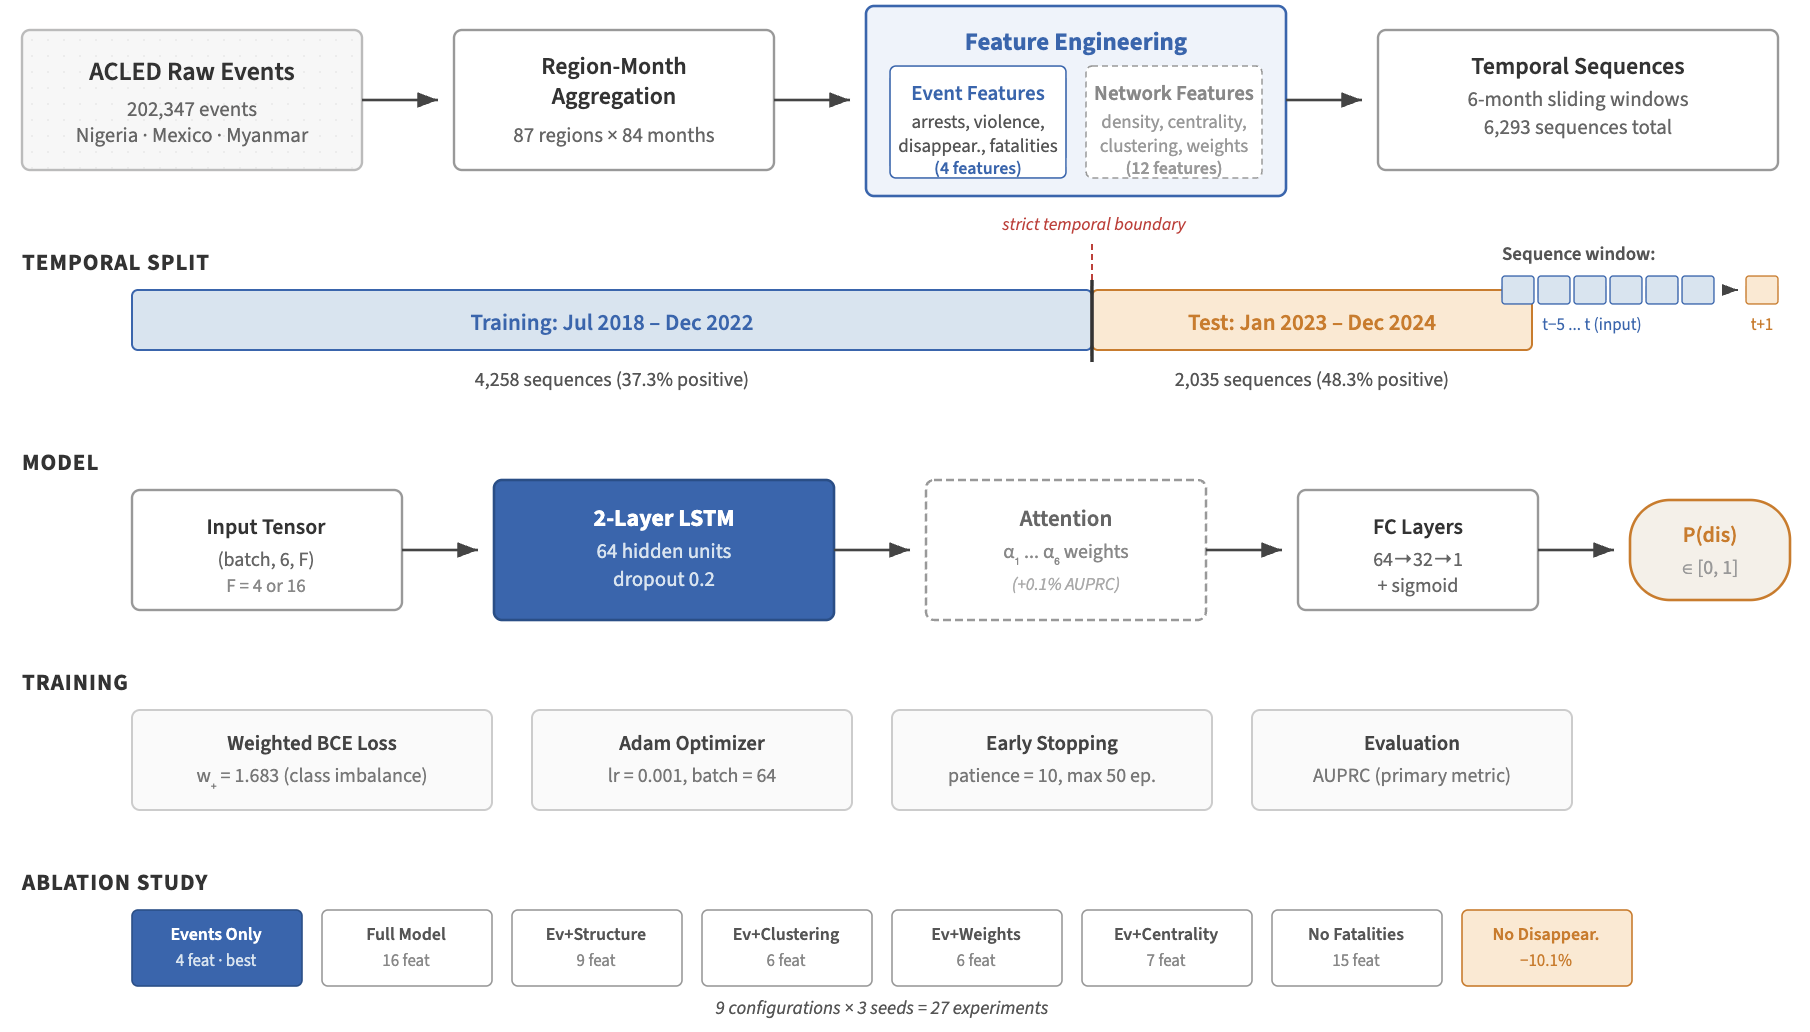
\includegraphics[width=\textwidth]{figures/pipeline_diagram.png}
\caption{End-to-end prediction pipeline. ACLED conflict events from Nigeria, Mexico, Myanmar, Afghanistan, and Syria (2018--2024) are aggregated to region-month units and transformed into event-based features (solid border) and actor network features (dashed border; 12 metrics providing no incremental predictive value beyond the event-based features in this dataset and design). Six-month sliding windows produce temporal sequences for LSTM processing. The temporal split separates training on 2018--2022 from evaluation on 2023--2024. Nine ablation configurations test feature contributions across 27 runs, three seeds each. The recommended model (Events Only, highlighted) uses 4 features and reaches test AUPRC 0.814, which is within 0.006 AUPRC of the seven best-performing configurations.}
\label{fig:pipeline}
\end{figure*}

\subsection{Data Collection and Preparation}

We analyze conflict event data from the Armed Conflict Location \& Event Data Project (ACLED), which provides geo-located, time-stamped records of political violence and protest events worldwide \cite{raleigh2010acled}. ACLED codes events from diverse sources, including local and international news, humanitarian reports, and NGO documentation, with each record containing location coordinates, administrative boundaries, event type, involved actors, fatality estimates, and descriptive text. Our analysis spans January 2018 through December 2024 and covers five countries selected through a principled multi-criteria approach. Because ACLED is event-report based, the outcome in this study should be read as reported disappearances rather than a direct census of all violations. We identify disappearance events using ACLED's \texttt{sub\_event\_type} field, coding events as disappearances when the sub-event type is \texttt{Abduction/forced disappearance}; the region-month outcome equals one if at least one such reported event occurs. ACLED analysts assign this sub-event type when a corroborated report -- drawn from local and international media, humanitarian organizations, and NGO documentation -- describes the deprivation of liberty of an identified individual or group whose fate remains unconfirmed at the time of coding, and every event additionally records the actor type(s) involved (state forces, rebel groups, political or identity militias, external forces, or unidentified armed groups) using ACLED's standard actor taxonomy \cite{raleigh2010acled}. This coding does not require that the perpetrator be a state actor: ACLED's \texttt{Abduction/forced disappearance} category is broader than the strict legal definition introduced in Section~\ref{sec:related}, which restricts enforced disappearance to acts committed by state agents or with state acquiescence \cite{icpped2006}. We do not filter events to isolate the subset meeting this narrower legal definition, since perpetrator attribution is frequently contested or unavailable at the point of reporting; the outcome modeled throughout this paper is therefore the broader, operationally defined \emph{abduction/forced-disappearance event}, not a verified legal determination. Two coding rules bound the category from the other side, and both work against our outcome rather than inflating it. ACLED applies an event-type hierarchy in which the most severe reported outcome determines the sub-event type, so an abduction whose victim is subsequently reported killed is coded as an attack and never enters our outcome; the cases that end in confirmed death are systematically absent. Deprivations of liberty carried out by non-state groups that operate a judicial or penal system are coded as arrests, which is one of our four predictor features rather than the outcome, placing a coding boundary between the target and one of its own inputs. Reporting environments are consequently part of the measurement process, and the outcome should be read as the reported subset of a larger and unobserved total.

Country selection balanced four considerations. First, we required enough recorded outcome events to support region-month modeling. Over the study window the five countries contribute 4,841 abduction/forced-disappearance events in Syria, 2,899 in Nigeria, 1,744 in Myanmar, 1,472 in Mexico, and 527 in Afghanistan. Mexico has documented a large number of disappeared persons since 1962, with 90\% occurring after 2006 during militarized anti-drug operations \cite{umnmexico2024}. Myanmar experienced systematic disappearances following the February 2021 military coup, targeting political opposition and civil society \cite{hrwmyanmar2021}. Nigeria exhibits disappearances across multiple conflict zones involving both insurgent groups and state security forces. Second, we sought geographic and contextual diversity to test whether findings hold across conflict types: state repression against political opposition in post-coup Myanmar, protracted civil war with large-scale detention in Syria, criminal violence with state involvement in Mexico's cartel war, multi-actor insurgency in Nigeria's Northeast, and insurgency followed by regime change in Afghanistan. The five sit in five world regions---West Africa, North America, Southeast Asia, the Middle East, and Central Asia. Third, they provide substantial subnational variation across 135 admin1 units: 37 in Nigeria, 34 in Afghanistan, 32 in Mexico, 18 in Myanmar, and 14 in Syria, ranging from units with no recorded disappearance in the training period to units with sustained monthly activity. Fourth, ACLED provides comparatively systematic coverage for all five countries throughout our study period, though coverage remains conditional on reporting environments and was checked for anomalous reporting gaps.

Two exclusions define the sampling frame, both recorded as named constants in \texttt{data\_prep.py}. ACLED assigns events at sea to maritime areas rather than to countries. These are not administrative units---no resident population, no admin1 geography---so the region-month unit of analysis is undefined for them, and the 149 such events in the export are dropped. Taiwan entered the extract as an artifact of the data pull rather than as a design choice: it records 6,190 events across 21 admin1 units and all 84 months, of which 6,093 are protests and none are abduction/forced disappearance. Retaining it would add 21 regions that are negative in every month, contributing 1,006 sequences of easily classified negatives. That leaves AUPRC effectively unchanged (0.8081 against 0.8088) while lifting AUROC by 3.1 points, from 0.8174 to 0.8483, and widening the margin over the persistence baseline by 1.4 points. Excluding Taiwan lowers the figures we report rather than raising them.

The window runs from January 2018 through December 2024, and its start is set by coverage comparability rather than by any country's own history. ACLED built its Latin America and Caribbean coverage out later than its Africa, Asia, and Middle East files, back-coding the region to the beginning of 2018 \cite{acledlac2020}; January 2018 is therefore the first month in which all five countries are covered on a comparable sourcing basis. An earlier start would produce a panel whose first years reflect the expansion of ACLED's monitoring in some countries and actual variation in violence in others, and the lagged event counts that carry most of the predictive signal would absorb that difference as trend. December 2024 is the end of the extract.

The five-country design is a purposive sample, not a random one. Contexts differing in state capacity, perpetrator type, and conflict intensity let us ask whether the limited utility of network features is a property of disappearance dynamics or an artifact of one setting, and the sample size keeps the nine-configuration ablation sweep with multiple seeds computationally tractable at admin1 resolution. Section~\ref{sec:results} reports per-country performance separately for this reason. Lift over each country's own prevalence holds in all five, which shows the result is not carried by a single case; it does not establish generalizability to the broader population of disappearance-affected settings, which requires validation in lower-prevalence and non-state-dominated contexts (Section~\ref{sec:discussion}).
% Future production systems require validating whether findings generalize to civil war contexts (Syria), post-conflict transitions (Colombia), and lower-prevalence settings, but this proof-of-concept isolates the question: can temporal models with simple features predict rare disappearances at operationally useful accuracy, and do complex network features add value? Our answer—yes to the first, no to the second—provides a baseline for broader validation efforts.

Our final dataset comprises 360,530 conflict events across 135 unique first-level administrative units (admin1 regions). These events include 11,483 abduction/forced-disappearance events (3.2\%), 8,371 arrests (2.3\%), 252,808 violent events including battles, explosions, and violence against civilians (70.1\%), and 438,917 total fatalities. Figure~\ref{fig:timeseries} shows the temporal distribution of disappearances across the five countries.

\begin{figure}[h]
\centering
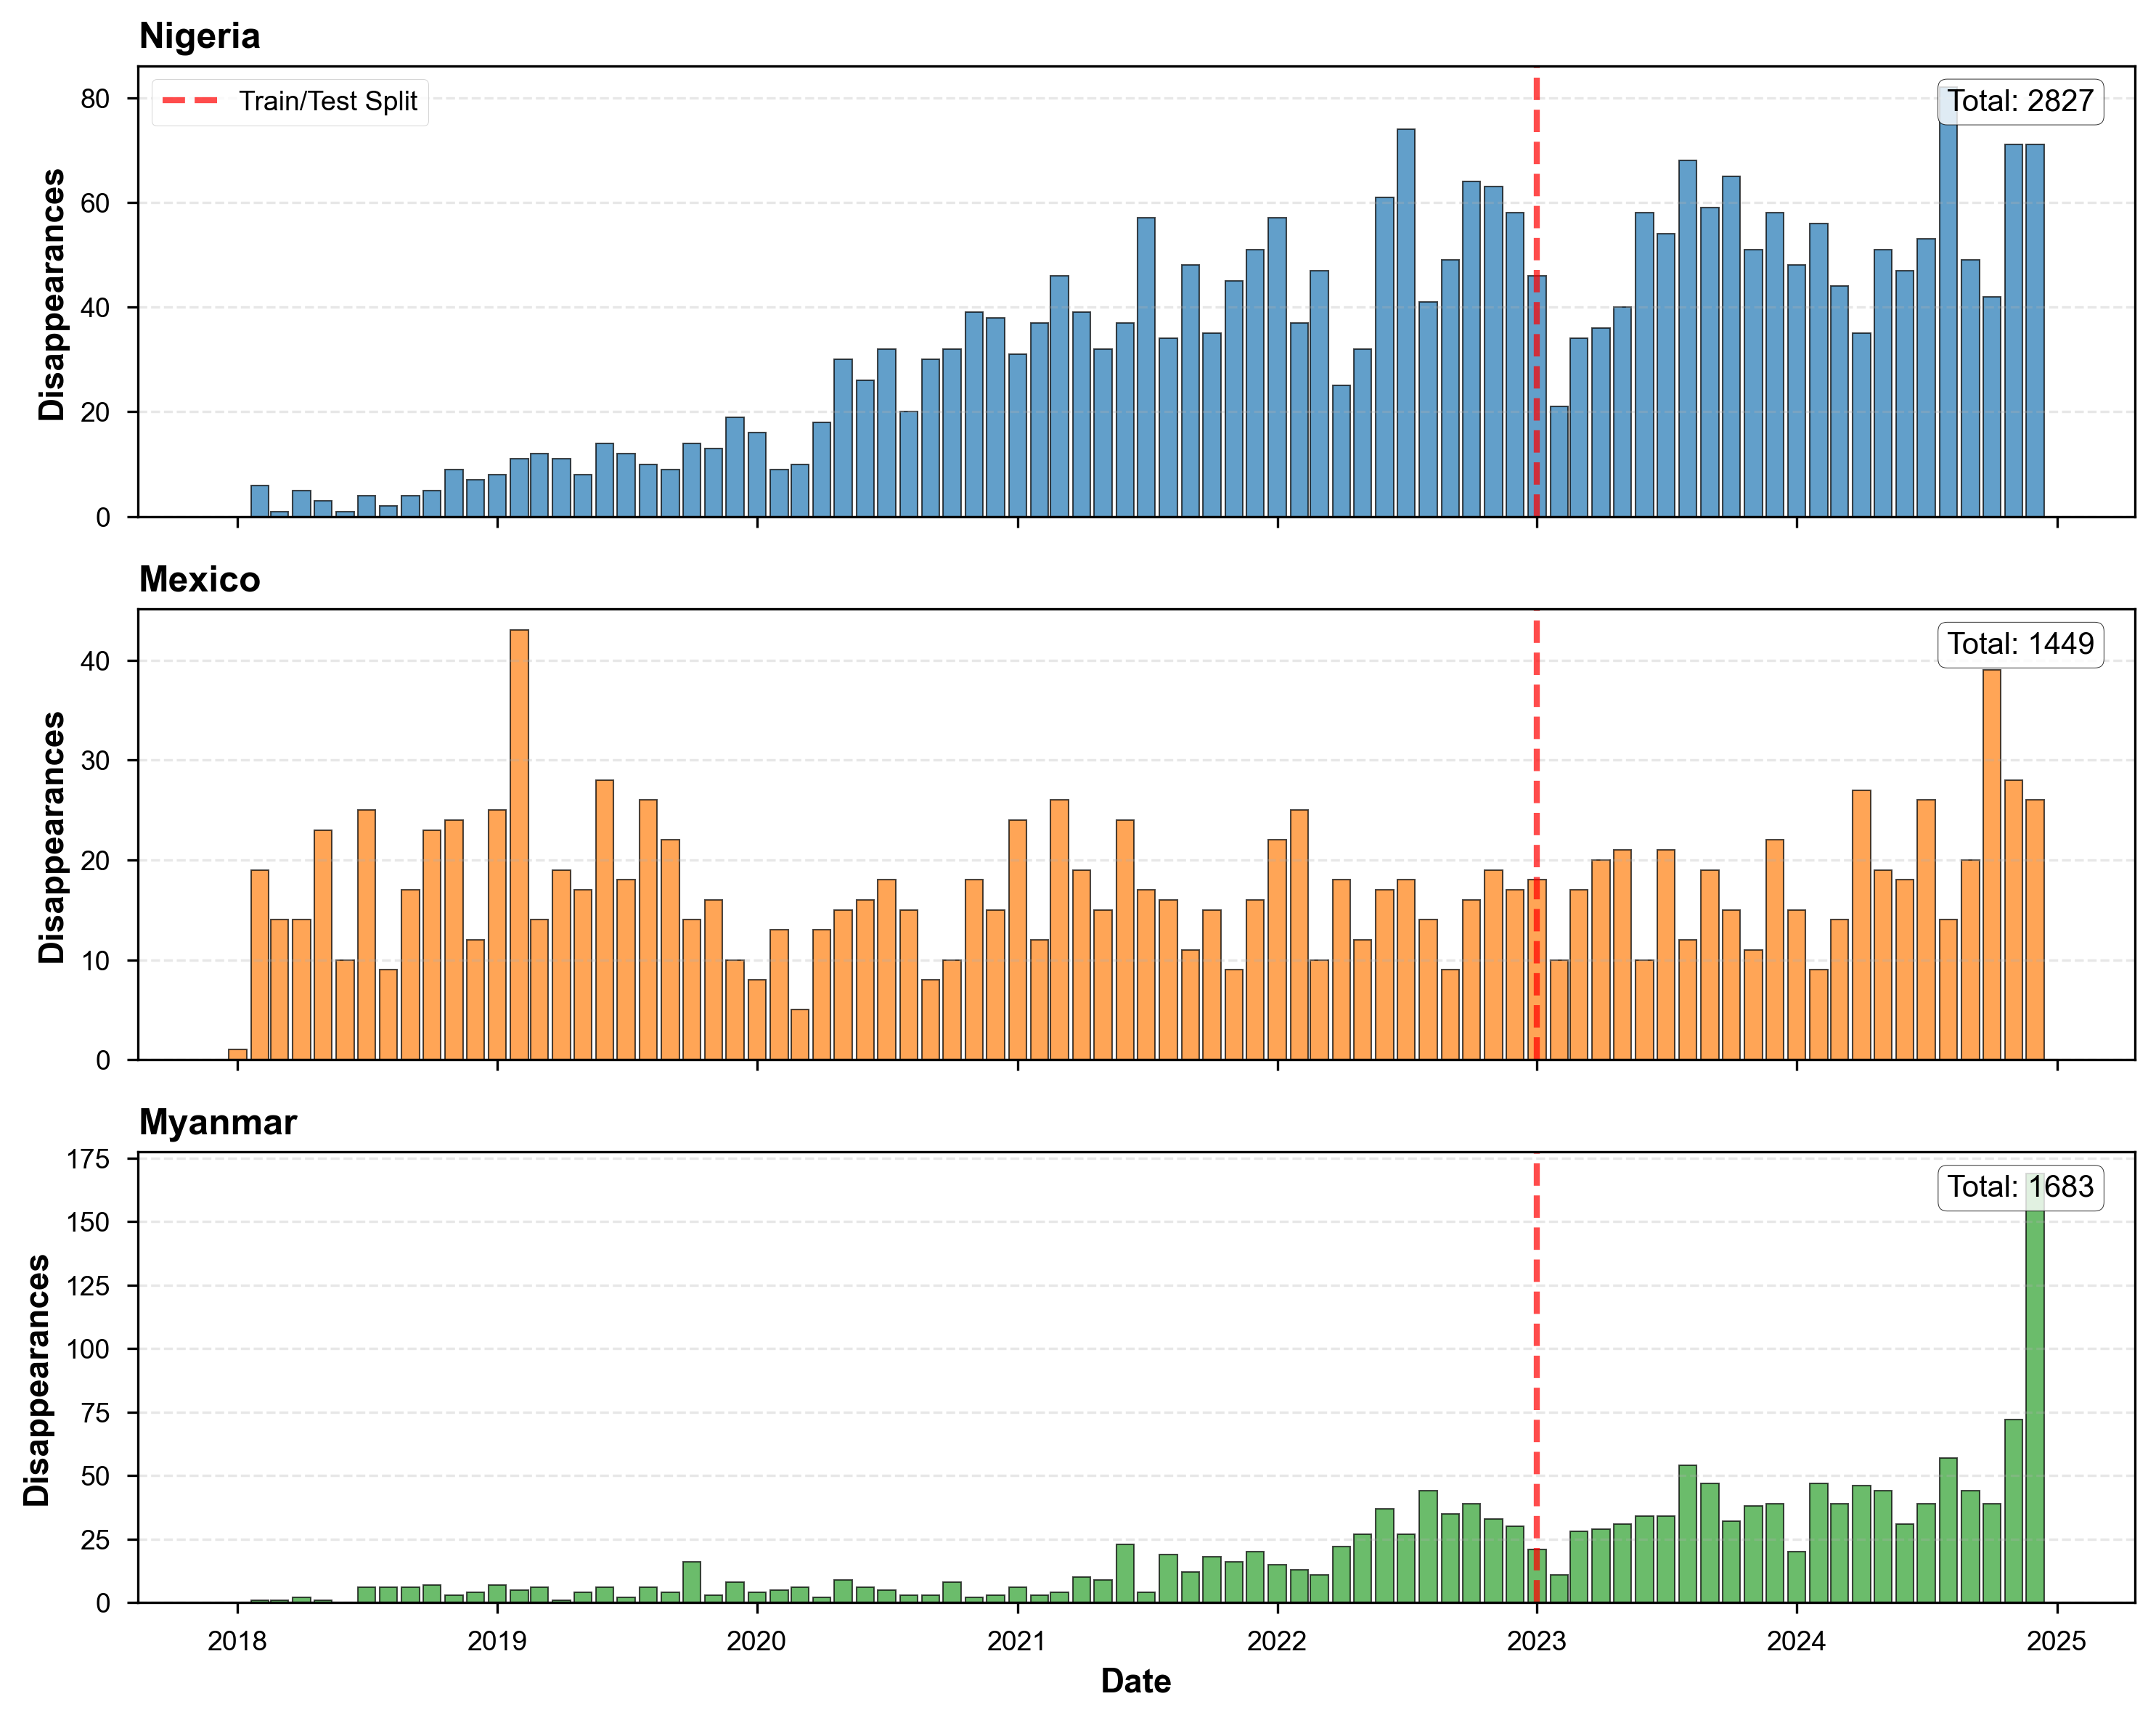
\includegraphics[width=\columnwidth]{figures/figure1_time_series.png}
\caption{Monthly disappearance events by country, 2018--2024. The vertical dashed line marks the train-test split boundary (January 2023). The test period carries a higher disappearance prevalence than the training period (45.9\% positive region-months against 31.1\%), a 14.8 point jump that reflects escalation across the study countries.}
\label{fig:timeseries}
\end{figure}

The unit of analysis is the admin1 region-month, and this is our design choice rather than one inherited from prior work. Subnational conflict forecasting operates predominantly at two other levels: the country-month and the fixed spatial grid cell, both used by the ViEWS ensemble \cite{hegre2019views, hegre2021views}. Admin1 sits between them, and we select it on grounds of data sufficiency that can be checked against the extract. ACLED codes administrative boundaries down to admin2, which would give 3,044 units in place of 135. At that resolution the median unit-month contains 2 events and 76.1\% of observed unit-months contain fewer than 5, so the actor co-occurrence networks from which all 12 network features are computed would be empty or trivial for most of the panel, and the panel itself would be 76\% unobserved cells. At admin1 the median unit-month contains 14 events, 24.8\% fall below 5, and 10,506 of the 11,340 possible region-months are observed. Admin1 also matches the level at which monitoring capacity and human-rights reporting are organized, so an alert corresponds to a jurisdiction rather than to a grid cell \cite{oswald2026googletrends}.

\subsection{Outcome Variable and Temporal Aggregation}

Following established practices in conflict prediction \cite{hegre2019views, ward2010perils}, we construct a binary outcome variable at the region-month level rather than modeling event counts. Our outcome $y_{i,t} \in \{0,1\}$ indicates whether region $i$ experienced at least one abduction/forced-disappearance event during month $t$. This binary formulation prioritizes outbreak detection---identifying which regions require monitoring attention---over precise victim enumeration, aligning with operational early warning requirements \cite{obrien2010crisis}.

This design choice reflects both substantive and methodological considerations. Operationally, early warning systems allocate limited monitoring resources across geographic units, requiring binary risk assessments rather than exact counts of cases. Substantively, disappearance counts suffer from severe underreporting, making presence/absence more reliably observed than precise magnitudes \cite{hrdag2024datasets}. Two prevalence figures appear in this paper and they differ by an order of magnitude. At the event level, abduction/forced disappearance accounts for 3.2\% of the 360,530 coded events, which is a statement about the phenomenon. At the region-month level, which is the classification task, 35.8\% of sequences are positive: 31.1\% in training and 45.9\% in test. Binary aggregation concentrates a signal that is sparse across events into a target that is not sparse across units, while preserving the discrimination the task requires, between affected and unaffected regions in a given month. Evaluation baselines follow the second figure, giving a prevalence-equivalent AUPRC baseline of 0.459 on the test period. Any reference to rarity in what follows is a reference to the event-level figure.

We considered and rejected the stronger argument that count targets are simply unpredictable in sparse settings. A supplementary Poisson regression on monthly counts (Section~\ref{sec:poisson_results}) reaches McFadden $R^2$ 0.36 and Lin's concordance correlation 0.47 on the test period, so counts in these data carry real signal and the binary target cannot be defended by denying it. The defense is operational instead. Test RMSE of 6.5 to 7.4 against a test MAE of 1.7 to 1.8 shows that count error is dominated by a small number of high-count months, which is the regime in which a magnitude estimate is least reliable and a threshold-crossing alert is most useful. The count target binarizes to the classification target with a match rate of 1.0, so the two analyses describe the same events at different resolutions.

\subsection{Feature Engineering}

We construct two feature categories capturing complementary aspects of conflict dynamics: event-based features that measure observable violence patterns, and network structure features that represent actor configurations. Table~\ref{tab:features} summarizes all 16 features with their theoretical motivations.

\begin{table*}[t]
\centering
\caption{Complete feature set with theoretical motivations. Event features capture directly observable conflict patterns; network features represent actor relationship structures within monthly region-specific co-occurrence networks.}
\label{tab:features}
\begin{tabular}{llp{7.5cm}}
\toprule
\textbf{Category} & \textbf{Feature} & \textbf{Theoretical Motivation} \\
\midrule
\multirow{4}{*}{Event-Based} 
& arrests & State repression capacity; precursor to disappearances \\
& violence & Overall conflict intensity; operational environment \\
& disappearances & Temporal persistence; campaign continuity \\
& fatalities & Severity of violence; escalation indicator \\
\midrule
\multirow{5}{*}{Structure} 
& num\_actors & Actor diversity; complexity of conflict landscape \\
& num\_edges & Interaction extent; level of engagement \\
& density & Connectivity saturation; integrated vs.\ fragmented \\
& num\_components & Network fragmentation; coalition structure \\
& largest\_component & Dominant coalition size; coordination capacity \\
\midrule
\multirow{3}{*}{Centrality} 
& avg\_degree & Typical connectivity level; diffuse vs.\ concentrated \\
& max\_degree & Most connected actor; potential dominance \\
& centralization & Concentration around hub; state capacity proxy \\
\midrule
\multirow{2}{*}{Clustering} 
& avg\_clustering & Local cohesion; neighborhood transitivity \\
& transitivity & Global cohesion; organized violence potential \\
\midrule
\multirow{2}{*}{Edge Weights} 
& avg\_edge\_weight & Typical interaction intensity; sustained engagement \\
& max\_edge\_weight & Strongest pairing; repeated confrontations \\
\bottomrule
\end{tabular}
\end{table*}

\subsubsection{Event-Based Features}

Event features quantify conflict dynamics directly observable in ACLED records. The \textit{arrests} feature counts events coded under ACLED's ``Strategic developments'' type with ``Arrests'' sub-event tag, capturing state repression activity that may precede disappearances. The \textit{violence} feature aggregates battles, explosions, and violence against civilians to measure overall conflict intensity. The \textit{disappearances} feature counts prior disappearance events within the same region-month, representing temporal autocorrelation and campaign continuity. The \textit{fatalities} feature sums reported deaths across all event types, indicating the severity of violence. These features reflect established findings that recent conflict history dominates prediction performance \cite{hegre2019views} and that process variables capturing recent events can substitute for structural factors over short forecasting horizons \cite{mueller2022hard}. These measures provide observable indicators of conflict activity, enabling us to evaluate their predictive contribution for disappearance forecasting.

\subsubsection{Network Structure Features}

For each region-month, we construct an actor co-occurrence network and extract twelve graph-theoretic features. This approach builds on work demonstrating that relational patterns improve conflict prediction \cite{dorff2020networks}, and tests whether these benefits extend to disappearance forecasting. Networks are constructed by treating unique armed actors (ACLED codes up to 2 actors per event) as nodes, with undirected edges connecting actor pairs that appear in the same event. Edge weights reflect co-occurrence frequency. Networks are constructed independently for each region-month using only events from that spatiotemporal unit. We implement network construction and feature extraction using NetworkX \cite{hagberg2007exploring}, with edge cases (empty networks or single actors) handled by returning zero-valued feature vectors.

From these monthly networks, we compute features across four categories. \textit{Basic structure features} quantify network size and connectivity: number of actors, number of edges, density (ratio of realized to possible connections), number of disconnected components, and largest component size. \textit{Centrality features} measure concentration: average degree (mean connections per actor), maximum degree (most connected actor), and degree centralization \cite{freeman1978centrality}. \textit{Clustering features} capture local cohesion: average clustering coefficient (neighborhood transitivity) and global transitivity (ratio of closed triads to connected triples). \textit{Edge weight features} measure interaction intensity: average and maximum co-occurrence frequencies.

The theoretical motivation for network features rests on several mechanisms. High centralization may indicate a dominant state actor with capacity for systematic repression. Multiple disconnected components may signal fragmentation creating unstable environments conducive to violations. High clustering may reflect organized violence by cohesive actor coalitions. High edge weights indicate sustained interactions between specific actor pairs. However, as Chadefaux and Schincariol \cite{chadefaux2025endogenous} demonstrate, complex features frequently fail to improve predictions over simple autoregressive models. Our ablation studies test whether these network features add predictive value specifically for disappearances.

\subsection{Temporal Sequence Construction and Train-Test Splitting}

We transform region-month features into fixed-length temporal sequences suitable for recurrent neural networks \cite{beck2000improving}. Each sequence comprises six consecutive months of features (months $t{-}5$ through $t$) paired with the binary outcome at month $t{+}1$. This sliding window approach generates one training example per region-month with sufficient history ($\geq 7$ months of data). For instance, predicting February 2023 disappearances in Lagos, Nigeria, uses feature vectors from August 2022 through January 2023 as input. We selected the 6-month lookback window to balance temporal context---capturing medium-term escalation patterns beyond single-month noise---with sample size constraints, as longer windows reduce usable sequences by requiring more historical data. This design follows best practices in conflict forecasting with temporal models \cite{malone2022recurrent, radford2022high}.

We employ strict temporal splitting to prevent data leakage and enable genuine out-of-sample evaluation \cite{hegre2017conflict}. The training period spans July 2018 through December 2022 (54 months), while the test period covers January 2023 through December 2024 (24 months), approximating a 70--30 temporal split. Unlike random cross-validation, this chronological division respects causality: models trained on past data predict future outcomes. All test sequences occur strictly after all training sequences, ensuring no future information contaminates model training. This split creates a realistic forecasting scenario in which the test period exhibits a distributional shift---45.9\% positive rate versus 31.1\% in training---reflecting an escalation in 2023--2024 disappearances across our study countries. Models must generalize across this shift. The temporal split and sequence construction are illustrated in the pipeline overview (Figure~\ref{fig:pipeline}, rows 1--2). Our final dataset comprises 9,696 sequences: 6,660 training sequences (31.1\% positive) and 3,036 test sequences (45.9\% positive).

Before model training, we normalize features using z-score standardization to zero mean and unit variance: $z = (x - \mu) / \sigma$. Critically, normalization parameters $\mu$ and $\sigma$ are computed exclusively on training data and applied to both training and test sets, preventing information leakage from test distribution into preprocessing \cite{lecun2012efficient}. Post-normalization, the training set exhibits a mean of 0.000 and a standard deviation of 1.000 by construction, while test statistics differ, reflecting the distributional shift.

\subsection{Model Architecture}

We evaluate two Long Short-Term Memory (LSTM) architectures: a standard LSTM baseline and an attention-augmented variant. Both models employ identical recurrent processing but differ in how they aggregate temporal information for final classification.

The standard LSTM processes input sequences of shape (batch size, 6 timesteps, $F$ features) through a 2-layer stacked LSTM with 64 hidden units per layer and dropout rate 0.2. At each timestep $t$, the LSTM computes hidden state $h_t = \text{LSTM}(x_t, h_{t-1}, c_{t-1})$ where $x_t$ is the feature vector, $h_{t-1}$ is the previous hidden state, and $c_{t-1}$ is the cell state. After processing all six timesteps, the final hidden state $h_6$ passes through a classification head: a fully connected layer reducing dimensionality from 64 to 32 with ReLU activation and dropout 0.2, followed by an output layer projecting to a single logit with sigmoid activation producing probability $\hat{y} \in [0,1]$. This architecture contains approximately 58,000 parameters.

The attention-LSTM extends this architecture by learning which months contribute most to predictions \cite{malhotra2015long}. Rather than using only $h_6$, it computes attention weights over all hidden states $h_1, \ldots, h_6$. For each timestep $t$, we compute attention score $e_t = W_2 \cdot \tanh(W_1 \cdot h_t)$ where $W_1$ and $W_2$ are learned weight matrices. These scores are normalized via softmax: $\alpha_t = \exp(e_t) / \sum_{i=1}^6 \exp(e_i)$, producing attention weights that sum to one. The context vector $c = \sum_{t=1}^6 \alpha_t h_t$ aggregates all hidden states weighted by their importance. This context vector then passes through the same classification head as the standard LSTM. The attention mechanism adds approximately 2,000 parameters, yielding ${\approx}$60,000 total. Beyond potential performance gains, attention provides interpretability: if $\alpha_6 \gg \alpha_1$, predictions rely primarily on the most recent month, while uniform weights indicate equal contribution across the lookback window. Both architectures are depicted in the model row of Figure~\ref{fig:pipeline}.

\subsection{Training Configuration and Optimization}

We train models using binary cross-entropy loss with class weighting to address the 31.1\% positive, 68.9\% negative imbalance in training data \cite{he2009learning}:

\begin{equation}
\mathcal{L} = -\frac{1}{N} \sum_{i=1}^N \bigl[w_+ \cdot y_i \log(\hat{y}_i) + w_- \cdot (1-y_i) \log(1-\hat{y}_i)\bigr]
\end{equation}

\noindent where $w_+ = (1-p)/p = 2.213$, computed from the unrounded training-set positive rate ($p \approx 0.311$), and $w_- = 1.0$. This weighting penalizes false negatives 2.213 times more severely than false positives, compensating for the underrepresentation of disappearances in training data.

We optimize using Adam \cite{kingma2015adam} with learning rate 0.001, batch size 64, and default momentum parameters ($\beta_1{=}0.9$, $\beta_2{=}0.999$). Training runs for a maximum of 50 epochs with early stopping based on evaluation loss, using a patience of 10 epochs. Regularization comes exclusively from dropout \cite{srivastava2014dropout} applied at rate 0.2 in both LSTM layers and fully connected layers; we do not employ L2 weight decay. All models train on CPU in 2--3 minutes per random seed using PyTorch 2.0, as the modest model size (${\approx}$60,000 parameters) and dataset size (9,696 sequences) make GPU acceleration unnecessary.

\subsection{Evaluation Metrics}

Following best practices for imbalanced classification \cite{saito2015precision}, we report multiple complementary metrics with primary emphasis on the Area Under the Precision-Recall Curve (AUPRC). The precision-recall curve plots precision ($\text{TP}/(\text{TP}+\text{FP})$) versus recall ($\text{TP}/(\text{TP}+\text{FN})$) across all decision thresholds, focusing exclusively on positive class performance. AUPRC summarizes this curve as a single scalar, with higher values indicating better classification.

We prioritize AUPRC over AUROC for three reasons. First, precision and recall depend only on true positives, false positives, and false negatives, making them insensitive to the large number of true negatives in our 45.9\% positive test set. AUROC's false-positive rate includes true negatives in its denominator, potentially yielding optimistic estimates when the majority class dominates. Second, random classifier performance differs meaningfully across metrics: AUPRC equals the positive class prevalence (0.459 in our test set), providing an informative baseline, whereas AUROC always equals 0.50 regardless of class balance. Third, for operational early warning systems, precision-recall tradeoffs directly correspond to policy-relevant questions about acceptable false alarm rates versus detection rates.

As secondary metrics, we report AUROC for comparison with prior work, Brier score measuring probability calibration ($\frac{1}{N}\sum_{i=1}^N(\hat{y}_i - y_i)^2$, lower is better), and precision-recall values at specific operating points for deployment scenario analysis.

\subsection{Ablation Study Design}

To identify which features drive predictive performance, we conduct comprehensive ablation studies testing nine feature configurations, with each configuration trained using three random seeds (42, 123, 456) for a total of 27 experiments. Table~\ref{tab:ablation_design} specifies all configurations and their purposes.

\begin{table}[h]
\centering
\caption{Ablation study configurations. All experiments employ identical training procedures (same seeds, hyperparameters, temporal split, early stopping) for fair comparison. Feature counts vary by configuration while total sequences (9,696) remain constant.}
\label{tab:ablation_design}
\begin{tabular}{lcp{5cm}}
\toprule
\textbf{Configuration} & \textbf{\# Feat.} & \textbf{Purpose} \\
\midrule
Full Model & 16 & Baseline with all features \\
Events Only & 4 & Quantify network contribution \\
Network Only & 12 & Quantify event contribution \\
No Disappearances & 15 & Measure autocorrelation dependency \\
No Fatalities & 15 & Test fatalities marginal value \\
Events + Structure & 9 & Isolate basic structure metrics \\
Events + Centrality & 7 & Isolate centrality metrics \\
Events + Clustering & 6 & Isolate clustering metrics \\
Events + Weights & 6 & Isolate edge weight metrics \\
\bottomrule
\end{tabular}
\end{table}

We maintain strict experimental control across all ablations. Each configuration uses identical random seeds, ensuring the same weight initializations and batch orderings. Hyperparameters remain fixed: learning rate 0.001, batch size 64, dropout 0.2, class weights 2.213/1.0. The train-test temporal split is identical (2018--2022 train, 2023--2024 test). All configurations use the same early-stopping procedure with a patience of 10 epochs. This control isolates feature composition as the sole experimental variable.

Our analysis strategy compares specific configuration pairs to answer targeted questions. Comparing Full Model versus Events Only quantifies network feature contribution by measuring performance change when removing all twelve network features. Comparing Full Model versus No Disappearances measures autocorrelation dependency, revealing how much performance derives from temporal persistence versus other predictive signals. Comparing Events Only versus each Events + [category] configuration tests whether specific network feature categories (structure, centrality, clustering, weights) add value when combined with event features. We report results as mean $\pm$ standard deviation across three random seeds. With only three replicates, we emphasize effect sizes and consistency across runs rather than formal significance testing. Differences exceeding one standard deviation and consistent across all three seeds are interpreted as meaningful.

% We additionally compare LSTM models to logistic regression to assess whether temporal modeling provides value over linear feature combinations. The logistic regression baseline uses identical features flattened to a single vector (6 timesteps $\times$ $F$ features dimensions), the same train-test temporal split, and class weighting (2.213 for positives), but employs default scikit-learn settings without hyperparameter tuning. If LSTM substantially outperforms logistic regression, it indicates that temporal structure---captured by recurrent connections across the 6-month lookback window---provides genuine predictive signal beyond linear combinations of lagged features \cite{king2001logistic}.
We additionally compare LSTM models to logistic regression to assess whether temporal modeling provides value over linear feature combinations. The logistic regression baseline uses identical features flattened to a single vector (6 timesteps $\times$ $F$ feature dimensions), the same train-test temporal split, and class weighting (2.213 for positives), but employs default scikit-learn settings without hyperparameter tuning. We also evaluate tuned non-temporal baselines and a persistence baseline, described in Section~\ref{sec:additional_baselines}.

\subsection{Additional Baselines}\label{sec:additional_baselines}

To ensure that performance differences reflect genuine temporal structure rather than insufficient baseline tuning, we evaluate three additional baselines: tuned logistic regression, XGBoost, and a naive persistence model.

For tuned logistic regression, we use \texttt{GridSearchCV} with \texttt{TimeSeriesSplit} ($n\_splits=5$) and \texttt{scoring=`average\_precision'}. The search grid includes regularization strength $C \in \{0.001, 0.01, 0.1, 1, 10, 100\}$, penalty $\in \{l1, l2\}$, and solver $\in \{\text{liblinear}, \text{saga}\}$, with class weights matching the LSTM configuration ($w_+ = 2.213$). Inputs are flattened identically to the untuned logistic regression baseline (6 timesteps $\times$ $F$ features). We evaluate both the Full Model configuration (16 features; 96 dimensions) and the Events Only configuration (4 features; 24 dimensions).

We also evaluate XGBoost as a gradient-boosted tree baseline using \texttt{GridSearchCV} with \texttt{TimeSeriesSplit} ($n\_splits=5$) and \texttt{scoring='average\_precision'}. The search grid includes \texttt{n\_estimators} $\in \{100, 300, 500\}$, \texttt{max\_depth} $\in \{3, 5, 7\}$, \texttt{learning\_rate} $\in \{0.01, 0.05, 0.1\}$, and \texttt{subsample} $\in \{0.8, 1.0\}$, with \texttt{scale\_pos\_weight} $= 2.213$. Inputs are flattened identically to the logistic regression baselines. XGBoost provides an independent test of the null finding for network features: if a tree-based model capable of capturing nonlinear feature interactions also gains nothing from network features, this null result is unlikely to arise from limitations specific to the LSTM or linear models.

Finally, we implement a naive persistence baseline defined as $\hat{y}(t{+}1) = y(t)$, where the prediction for the next month equals whether disappearances occurred in the most recently observed month. This baseline requires no training and provides a standard sanity check in conflict forecasting \cite{hegre2024views}, establishing the minimum performance threshold that a model must exceed to demonstrate value beyond simple autocorrelation.

\subsection{Supplementary Regression Analysis}\label{sec:poisson_methods}

The binary classification task asks whether a region-month will record at least one disappearance. As a complement, we fit a Poisson regression on the raw disappearance count in the target region-month, using the same 6-month input window flattened identically (96 dimensions for the Full Model, 24 for Events Only) and the same temporal train/test cutoff (train through 2022-12, test from 2023-01). We use an L2-penalized Poisson generalized linear model with a log link (scikit-learn's \texttt{PoissonRegressor}), tuning the regularization strength $\alpha \in \{0.001, 0.01, 0.1, 1, 10, 100\}$ via \texttt{GridSearchCV} with \texttt{TimeSeriesSplit} ($n\_splits=5$), scoring on negative mean Poisson deviance. We report mean absolute error (MAE), root mean squared error (RMSE), mean Poisson deviance, McFadden pseudo-$R^2$ against an intercept-only null model fit on the training mean rate, and Lin's concordance correlation coefficient (CCC), following the regression-evaluation framework of Correndo et al.~\cite{correndo2022metrica}. This analysis checks whether the binary framing conceals count-level signal; it is not a replacement for it, since our motivating use case (Section~\ref{sec:related}) is an early-warning trigger rather than a magnitude forecast.

\subsection{Reproducibility}

To facilitate replication and extension, we will release complete code, environment specifications, and trained models upon publication. Our GitHub repository will contain Python implementations of all preprocessing pipelines, feature engineering, model architectures, training procedures, and evaluation scripts, with exact package versions specified (PyTorch 2.0.1, NumPy 1.24.3, Pandas 2.0.2, NetworkX 3.1, scikit-learn 1.3.0). All experiments use fixed random seeds (42, 123, 456) for deterministic replication. ACLED data are publicly available at \url{https://acleddata.com/} with free registration.

This research uses publicly available conflict event data and does not involve human subjects. All analysis focuses on aggregate regional patterns rather than individual identification. Code and data sharing follows ACLED's terms of use permitting academic research with proper attribution.

\section{Results}\label{sec:results}

We present results in three stages: model architecture comparison, systematic feature ablations, and country-level performance. All metrics represent mean ± standard deviation across three random seeds (42, 123, 456). Figure~\ref{fig:ablations} provides a visual overview of ablation results.

\begin{figure*}[t]
\centering
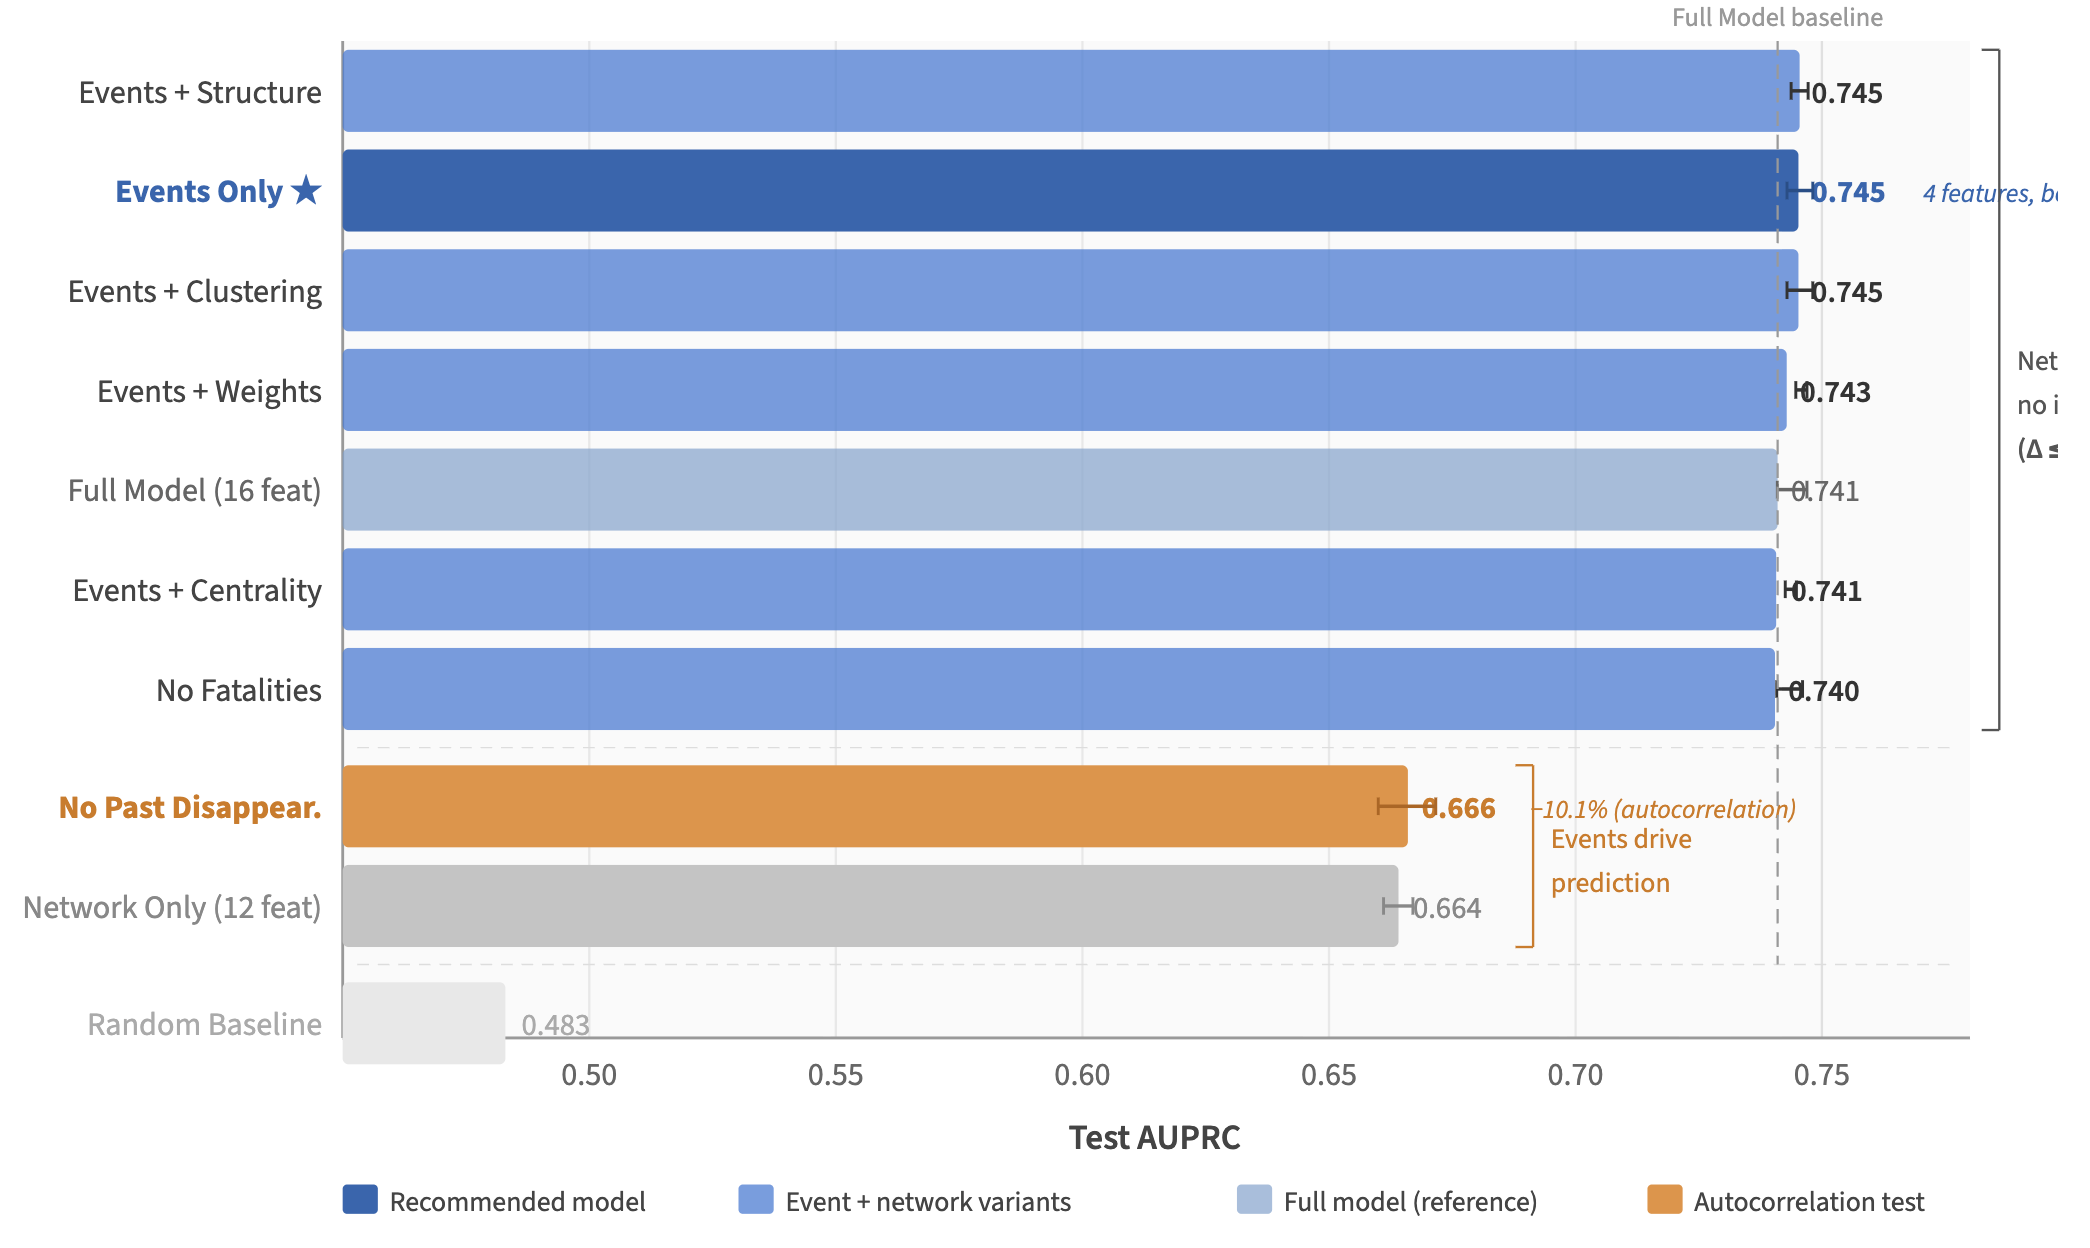
\includegraphics[width=\textwidth]{figures/ablation_chart.png}
\caption{Feature ablation study results sorted by test AUPRC (mean $\pm$ SD across 3 random seeds). The Events Only model (4 features) ranks first, ahead of every network-augmented configuration including the Full Model with 16 features; adding any single network category costs 0.001--0.002 AUPRC. The dashed vertical line marks the Full Model baseline. Removing past disappearances causes the largest single drop (a quarter of the gain over the random baseline), leaving 0.723 against a random baseline of 0.459; Section~\ref{sec:zero_history} shows that predictive skill was not demonstrated for regions without training-period history.}
\label{fig:ablations}
\end{figure*}

\subsection{Model Architecture Comparison}

Table~\ref{tab:model_comparison} compares LSTM architectures against baselines on the full 16-feature set.

\begin{table}[h]
\centering
\caption{Performance comparison of model architectures on the full 16-feature set, sorted by test AUPRC. LSTM models trained with 3 random seeds; tuned LR, XGBoost, and untuned logistic regression with a single run each. Persistence baseline uses $\hat{y}(t+1) = y(t)$. Random baseline equals test set prevalence (45.9\%). Gap = Train $-$ Test AUPRC, so a negative value means the model scores higher on the test period than on the training period.}
\label{tab:model_comparison}
\small
\begin{tabular}{lcccc}
\toprule
\textbf{Model} & \textbf{Test AUPRC} & \textbf{Train AUPRC} & \textbf{Gap} & \textbf{Brier} \\
\midrule
Tuned LR & 0.811 & 0.736 & $-0.075$ & 0.182 \\
Standard LSTM & 0.809 $\pm$ 0.001 & 0.758 & $-0.051$ & 0.181 $\pm$ 0.001 \\
Logistic Regression (untuned) & 0.809 & 0.738 & $-0.071$ & 0.183 \\
Attention-LSTM & 0.808 $\pm$ 0.002 & 0.764 & $-0.044$ & 0.186 $\pm$ 0.004 \\
XGBoost & 0.792 & 0.742 & $-0.051$ & 0.195 \\
Persistence Baseline & 0.597 & --- & --- & 0.307 \\
Random Baseline & 0.459 & --- & --- & --- \\
\bottomrule
\end{tabular}
\end{table}

Five of the seven rows are separated by less than 0.02 AUPRC. Both LSTM models reach test AUPRC ${\approx}$0.81, which is 34.9 points above the random baseline and 21.1 points above persistence, and neither leads the table: a tuned logistic regression scores 0.811 and an untuned one 0.809. XGBoost is the weakest of the learned models at 0.792. Recurrent architecture therefore buys nothing measurable over a linear model on flattened windows, a point we test directly below.

Every model scores higher on the test period than on the training period (gaps of $-0.044$ to $-0.075$). This reflects the shift in outcome prevalence between the two periods, from 31.1\% positive region-months in training to 45.9\% in test, and it is not evidence about generalization: the largest test-over-train gain belongs to the tuned logistic regression, not to either LSTM. We retain Attention-LSTM for the ablations because its attention weights support the temporal attribution in Section~\ref{sec:temporal_attribution}, not because it predicts better.

The 0.003 AUPRC separation between Attention-LSTM and tuned LR in Table~\ref{tab:model_comparison} runs in the linear model's favour and is small enough to require its own test before being read either way. We compare the Attention-LSTM's three-seed ensemble-averaged test probabilities against tuned LR's probabilities on the identical test set ($n=3036$) using two paired resampling procedures: a bootstrap over test sequences (10,000 resamples with replacement) and a permutation test that independently reassigns, for each test sequence, which model's predicted probability is treated as which (10,000 permutations). On the full 16-feature set the observed difference is $-0.001$ in the LSTM's direction, the bootstrap 95\% confidence interval is $[-0.006, +0.005]$, and the permutation test gives a two-sided $p=0.805$. Repeating the procedure on the events-only specification, which is the configuration we recommend, gives an observed difference of $+0.003$ favouring the LSTM, a confidence interval of $[-0.000, +0.006]$ that still includes zero, and $p=0.444$. Neither feature set separates the two model families.

\subsection{Feature Ablation Results}

Table~\ref{tab:ablation_results} presents systematic ablations testing nine feature configurations.

\begin{table}[h]
\centering
\caption{Feature ablation study results sorted by test AUPRC. $\Delta$ indicates change relative to the Full Model (16-feature) baseline. \#F = number of input features. All experiments use Attention-LSTM with identical seeds, hyperparameters, and temporal split.}
\label{tab:ablation_results}
\small
\begin{tabular}{clccc}
\toprule
\textbf{Rank} & \textbf{Configuration} & \textbf{Test AUPRC} & \textbf{$\Delta$} & \textbf{\#F} \\
\midrule
1 & \textbf{Events Only} & \textbf{0.814 $\pm$ 0.000} & \textbf{+0.005} & \textbf{4} \\
2 & Events + Clustering & 0.813 $\pm$ 0.000 & +0.004 & 6 \\
3 & Events + Structure & 0.813 $\pm$ 0.001 & +0.004 & 9 \\
4 & Events + Centrality & 0.813 $\pm$ 0.001 & +0.004 & 7 \\
5 & Events + Weights & 0.812 $\pm$ 0.001 & +0.003 & 6 \\
6 & Full Model & 0.809 $\pm$ 0.001 & --- & 16 \\
7 & No Fatalities & 0.808 $\pm$ 0.001 & $-$0.001 & 15 \\
8 & \textbf{No Disappearances} & \textbf{0.723 $\pm$ 0.003} & \textbf{$-$0.086} & \textbf{15} \\
9 & Network Only & 0.693 $\pm$ 0.005 & $-$0.116 & 12 \\
\midrule
& \textit{Random Baseline} & \textit{0.459} & \textit{$-$0.349} & --- \\
\bottomrule
\end{tabular}
\end{table}

Table~\ref{tab:ablation_results} and Figure~\ref{fig:ablations} separate the nine configurations into one dense band and two isolated points. Ranks 1--7 span 0.808 to 0.814, a range of 0.006, and comprise every configuration that includes the four event-based features, whatever network features are added or removed alongside them. Rank 8 withholds past disappearances and falls to 0.723. Rank 9 keeps only the twelve network features and falls to 0.693, which is still 23.4 points above the 0.459 random baseline. Membership in the top band is decided by the presence of the event-based features and by nothing else in the design.

Three key findings emerge from ablations. First, events-only outperforms the full model, indicating the twelve tested network structure features provide no incremental predictive value beyond the event-based features in this dataset and design. If actor network configuration carried strong predictive signal for disappearances, removing network features would materially reduce predictive performance. We observe no such reduction. This holds for each network category taken on its own. Added to the four event features, clustering and structure each cost 0.001 AUPRC, centrality costs 0.001, and edge weights cost 0.002; none of the four improves on the event features alone. Events-only exceeds network-only by 12.1 points while using one-third as many inputs.

Second, removing past disappearances reduces AUPRC from 0.809 to 0.723, an 8.6-point drop and a quarter of the model's gain over the random baseline, which makes the lagged outcome the strongest single predictor. What remains without it is 26.3 points above random and 12.6 points above persistence, so arrests, violence, and fatalities carry predictive information that is not a restatement of the region's own disappearance history. That margin is measured over the whole test set, and the next subsection tests whether that margin extends to regions without such a history.

Third, removing fatalities changes AUPRC from 0.809 to 0.808, placing fatality counts within seed variation of redundancy with violence event counts.

\subsection{Regions Without Training-Period History}\label{sec:zero_history}

Withholding the lagged disappearance feature is necessary to rule out autocorrelation, but it is not sufficient: the No Disappearances configuration is still trained and evaluated on a panel dominated by regions that had disappearances during the training period, and it can learn the covariate signature of those regions. We therefore evaluate that configuration separately on the subset of regions where the training period contains no disappearance at all. Eight of 135 admin1 regions qualify: Badghis, Laghman, Nimruz and Paktika in Afghanistan, Ayeyarwady and Nay Pyi Taw in Myanmar, and Lattakia and Tartous in Syria. They contribute 160 test sequences with a 17.5\% positive rate.

On that subset the model reaches AUPRC 0.139 $\pm$ 0.010 against a no-skill baseline of 0.175, while the same three fitted models score 0.719 $\pm$ 0.010 across the full test set. The point estimate is below the no-skill baseline; given the limited subset of 160 sequences and 28 positives, predictive skill is not demonstrated. The 12.6-point margin over persistence reported above comes from regions that have a history. The distinction matters for how the model can be used: it ranks risk among places where disappearances have already been recorded, and predictive skill was not demonstrated on this limited subset of places where they have not.

Table~\ref{tab:events_only_comparison} shows that the network null finding is not specific to the LSTM architecture. Across all three model families, the Events Only configuration matches or outperforms the Full Model. The XGBoost Full Model shows the largest penalty from including network features ($-0.013$), suggesting that even a tree-based model capable of capturing non-linear interactions between network metrics gains nothing from them. This cross-model replication strengthens the conclusion that the tested graph-theoretic features derived from actor co-occurrence networks carry no incremental predictive value beyond the event-based features for disappearance forecasting in this dataset and design.

\begin{table}[h]
\centering
\caption{Events Only versus Full Model test AUPRC across model families. In all cases, removing the twelve network features maintains or improves predictive performance, replicating the network null finding across model architectures.}
\label{tab:events_only_comparison}
\small
\begin{tabular}{lccc}
\toprule
\textbf{Model} & \textbf{Events Only} & \textbf{Full Model} & \textbf{Difference} \\
\midrule
Attention-LSTM & 0.814 $\pm$ 0.000 & 0.809 $\pm$ 0.001 & $+0.005$ \\
Tuned LR & 0.812 & 0.811 & $+0.001$ \\
XGBoost & 0.805 & 0.792 & $+0.013$ \\
\bottomrule
\end{tabular}
\end{table}

\subsection{SHAP Feature Attribution}\label{sec:temporal_attribution}

To examine what the model has learned, we apply SHAP analysis (GradientExplainer, 3 seeds) to the Events Only Attention-LSTM. SHAP values are computed over the full test set (3,036 sequences) and averaged across seeds, yielding an output of shape $[3036 \times 6 \times 4]$ (sequences $\times$ timesteps $\times$ features).

Table~\ref{tab:shap_importance} reports mean absolute SHAP values per feature, averaged over all timesteps. Prior disappearances dominate with a mean $|\text{SHAP}|$ of 0.313, 15 times the next largest feature. The other three separate by very little: arrests 0.021, violence 0.017, fatalities 0.016, a range narrow enough that their ordering should not be read as a ranking. Attribution and ablation do not agree on how much the lagged feature matters, since withholding it costs 0.086 AUPRC, a quarter of the model's gain over the baseline rather than the near-totality its attribution share would imply.

\begin{table}[h]
\centering
\caption{Mean absolute SHAP values per feature, averaged over timesteps and seeds.}
\label{tab:shap_importance}
\small
\begin{tabular}{lcc}
\toprule
\textbf{Feature} & \textbf{Mean $|\text{SHAP}|$} & \textbf{Direction} \\
\midrule
Prior disappearances & 0.313 & Positive \\
Arrests              & 0.021 & Mixed \\
Violence             & 0.017 & Positive \\
Fatalities           & 0.016 & Positive \\
\bottomrule
\end{tabular}
\end{table}

Figure~\ref{fig:shap_heatmap} shows mean absolute SHAP values across all six lookback months and four features. The most recent month ($t$) contributes a mean $|\text{SHAP}|$ of 0.439 for disappearances, 1.6 times that of the oldest lookback month ($t-5$, mean $|\text{SHAP}|$ = 0.270). Summed across features the same gradient runs from 0.079 at $t-5$ to 0.133 at $t$, and it is not monotone: attribution dips at $t-3$ (0.072) before rising through the final two months. The model distributes weight across the window with a recency tilt rather than reading a single lag.

\begin{figure}[h]
\centering
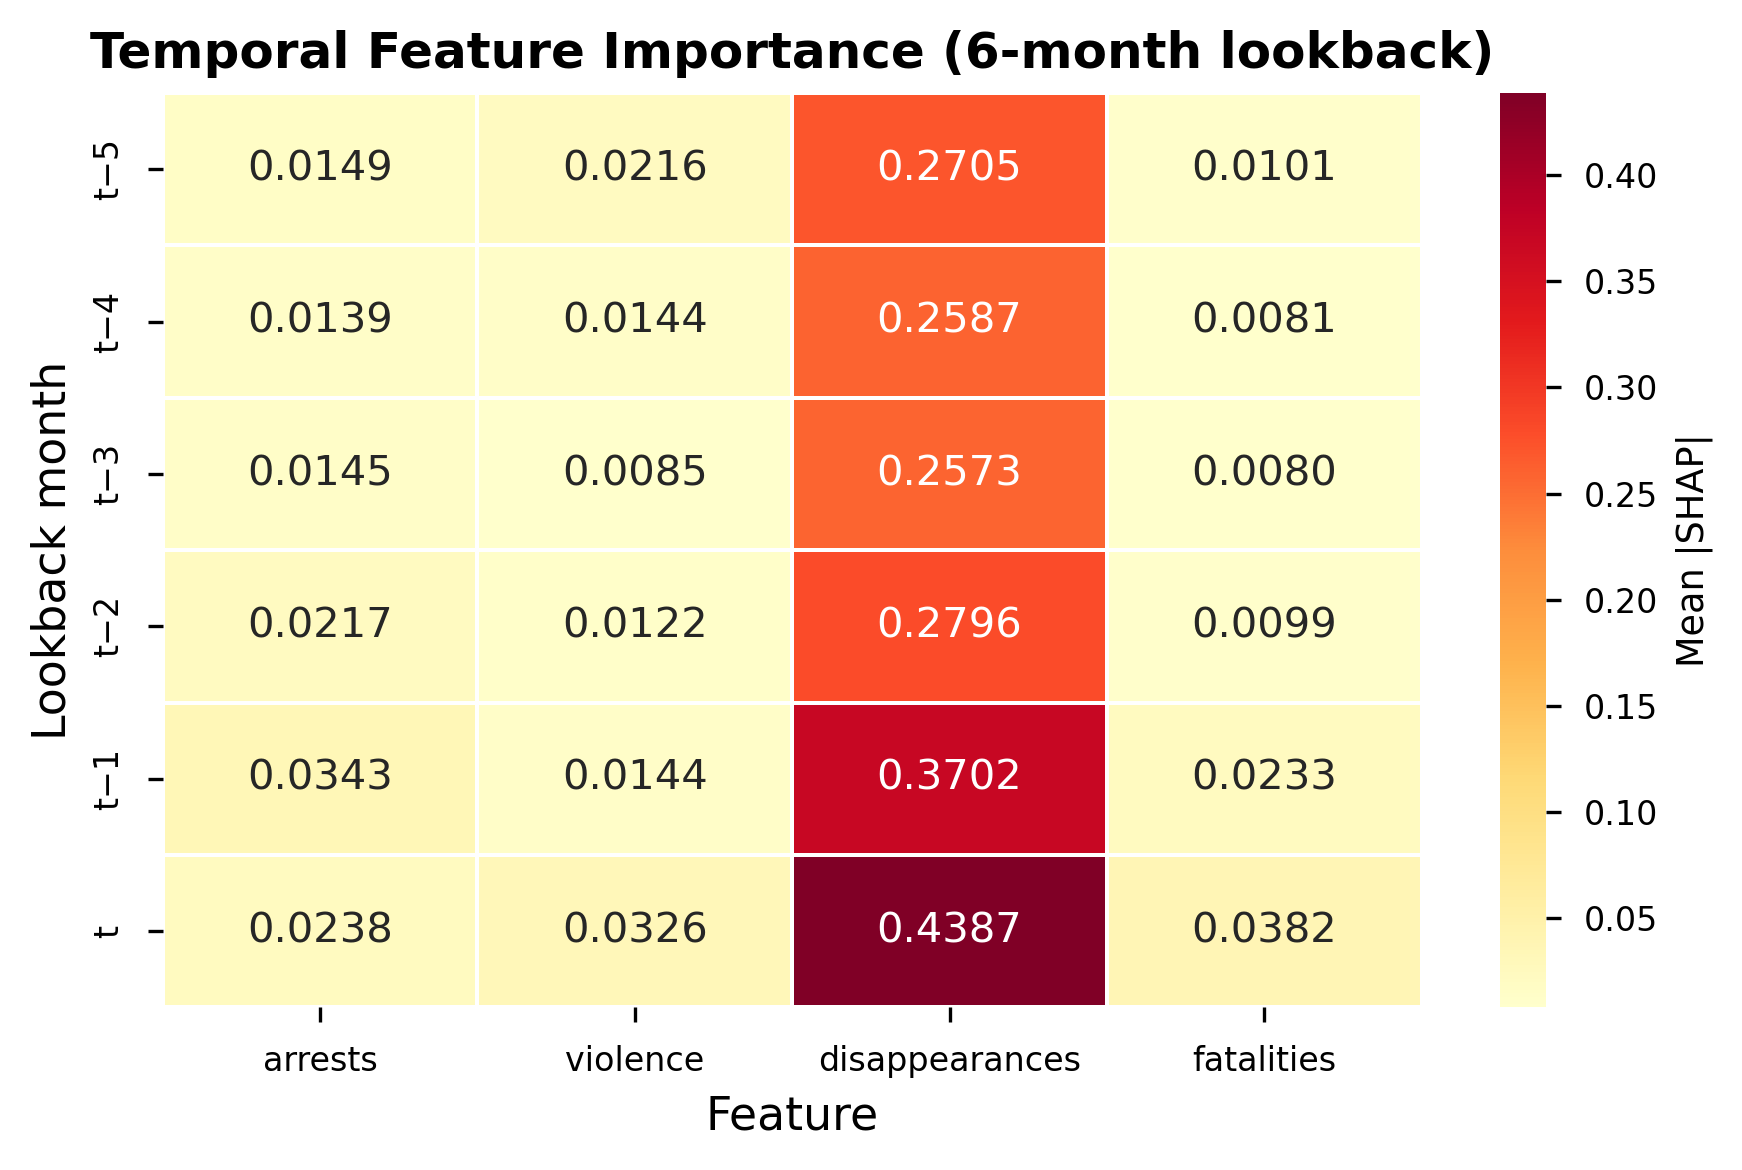
\includegraphics[width=0.85\textwidth]{figures/fig2_shap_heatmap.png}
\caption{Temporal feature importance across the 6-month lookback window. Color intensity reflects mean $|\text{SHAP}|$ value. Prior disappearances dominate across all timesteps, with a recency tilt at month $t$.}
\label{fig:shap_heatmap}
\end{figure}

Figure~\ref{fig:shap_direction} reveals an important nuance in the directional effects of arrests. While violence, disappearances, and fatalities show consistently positive SHAP values across all timesteps, arrests exhibit negative signed SHAP values at older timesteps ($t-5$ to $t-2$) and turn positive only at $t-1$ and $t$. This suggests the model has learned that recent arrest activity increases disappearance risk, while older arrest patterns carry a different and potentially stabilizing signal.

\begin{figure}[h]
\centering
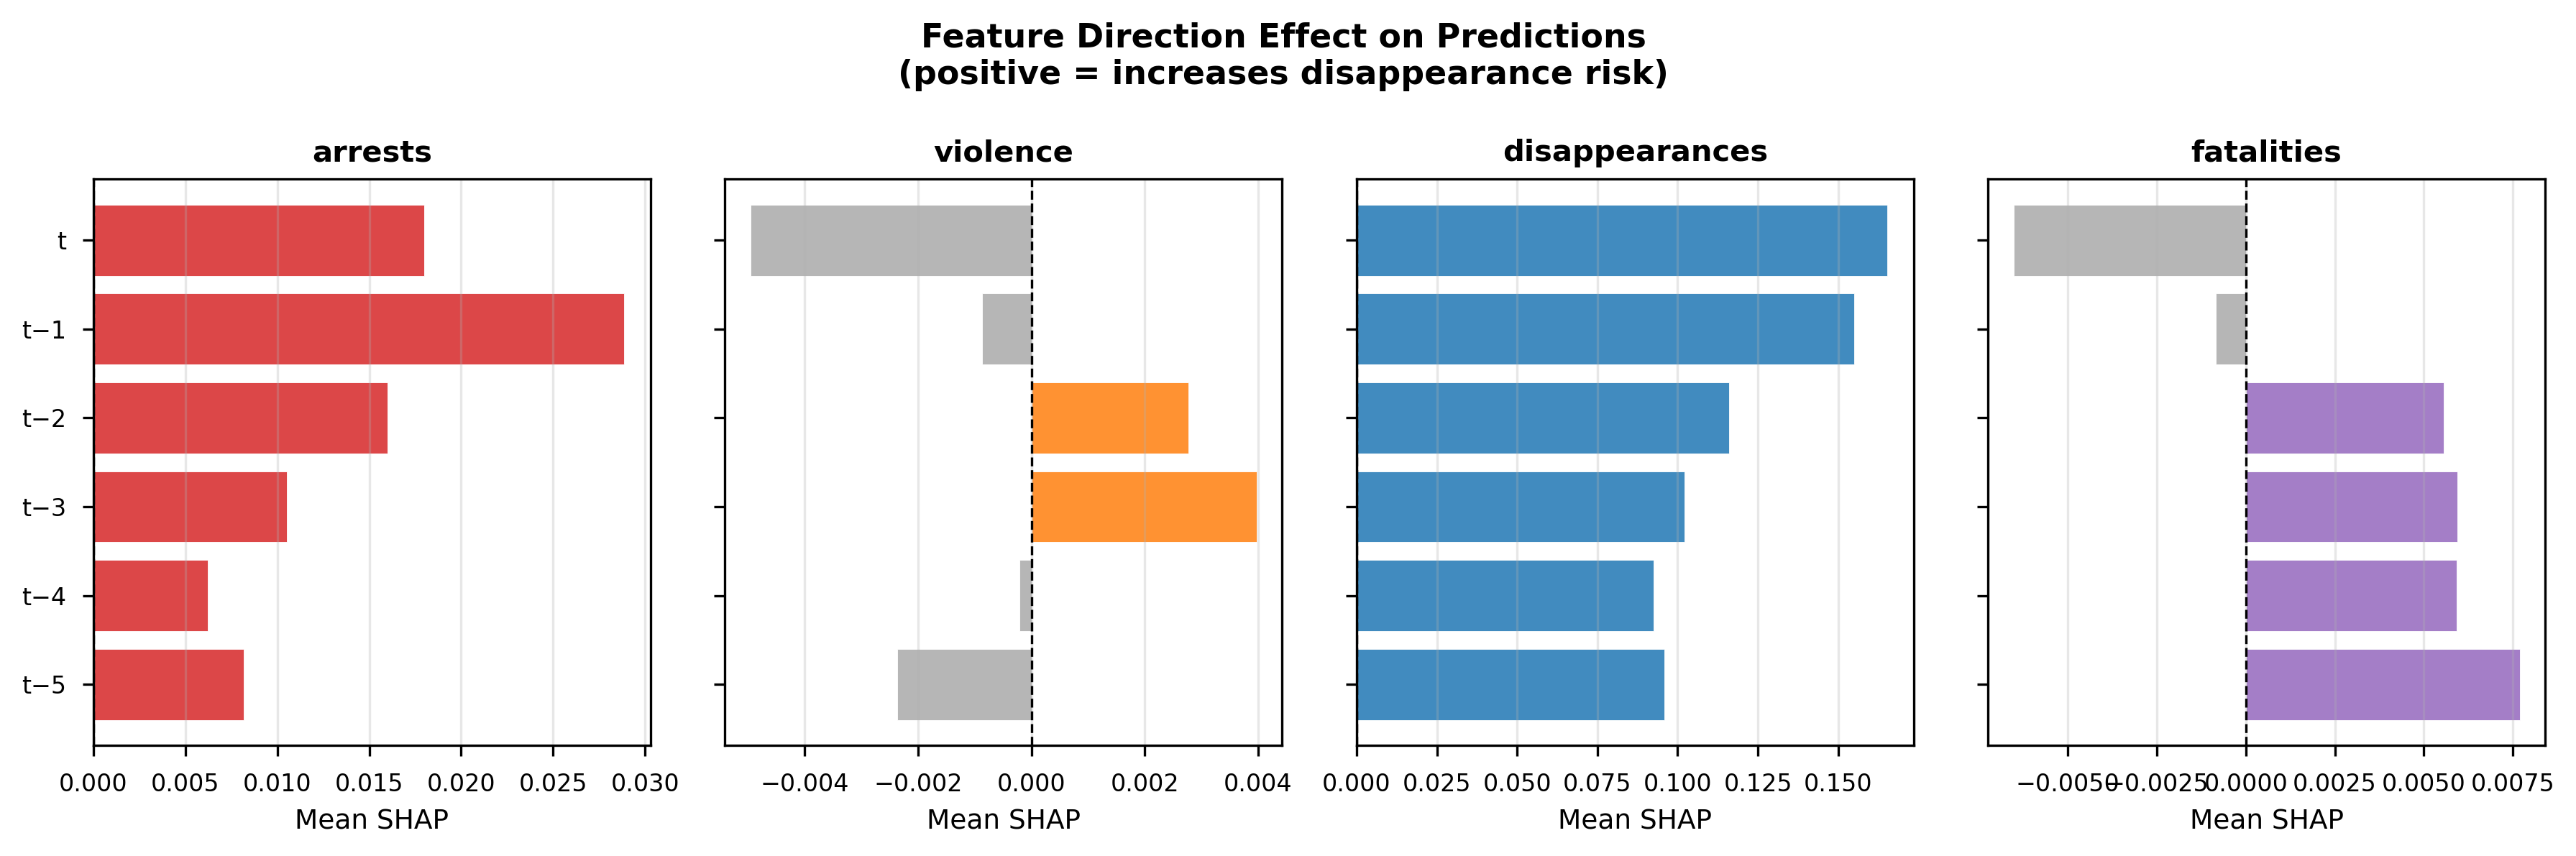
\includegraphics[width=0.95\textwidth]{figures/fig3_shap_direction.png}
\caption{Signed mean SHAP values per feature across the 6-month lookback window. Positive values indicate features that increase predicted disappearance risk. Arrests show a sign reversal between older and more recent timesteps.}
\label{fig:shap_direction}
\end{figure}

\subsection{Recommended Model}

Based on ablation results, we recommend the Events Only Attention-LSTM as the optimal configuration:

\begin{table}[h]
\centering
\caption{Recommended model specification achieving best test performance with fewest features.}
\label{tab:recommended}
\small
\begin{tabular}{ll}
\toprule
\textbf{Property} & \textbf{Specification} \\
\midrule
Architecture & 2-layer Attention-LSTM, 64 hidden units \\
Features & arrests, violence, disappearances, fatalities \\
Feature count & 4 (vs 16 for Full Model) \\
Test AUPRC & 0.814 $\pm$ 0.000 \\
Parameters & ${\approx}$55,000 \\
\bottomrule
\end{tabular}
\end{table}

This model achieves marginally better performance (+0.005 AUPRC) with 75\% fewer features, removes the actor-network construction step from the pipeline, and depends on four monthly counts that a monitoring organisation can read directly off an event feed. We did not test sensitivity to data quality, so no claim is made on that dimension.

\subsection{Country-Level Performance}

Table~\ref{tab:country} reports the pooled Events Only model scored separately within each country's test sequences; these are not per-country models. Raw AUPRC is not comparable across the five countries, because each country's no-skill baseline is its own test prevalence and that ranges from 0.232 in Afghanistan to 0.637 in Myanmar. Lift over own prevalence is the comparable quantity.

\begin{table}[h]
\centering
\caption{Country-level performance of the Events Only model. One pooled model per seed, scored within each country's test sequences. Lift is AUPRC minus that country's test positive rate, which is the no-skill AUPRC for that subset. Means across three seeds.}
\label{tab:country}
\small
\begin{tabular}{lccccc}
\toprule
\textbf{Country} & \textbf{Regions} & \textbf{Test seq.} & \textbf{Pos.\ rate} & \textbf{AUPRC} & \textbf{Lift} \\
\midrule
Afghanistan & 34 & 674 & 23.2\% & 0.571 & $+0.340$ \\
Mexico & 32 & 757 & 36.2\% & 0.595 & $+0.233$ \\
Myanmar & 18 & 419 & 63.7\% & 0.894 & $+0.256$ \\
Nigeria & 37 & 861 & 57.1\% & 0.804 & $+0.233$ \\
Syria & 14 & 325 & 63.4\% & 0.960 & $+0.326$ \\
\midrule
\textbf{Overall} & \textbf{135} & \textbf{3,036} & \textbf{45.9\%} & \textbf{0.814} & $\mathbf{+0.355}$ \\
\bottomrule
\end{tabular}
\end{table}

Raw AUPRC spans 38.9 points across the five countries, from 0.571 in Afghanistan to 0.960 in Syria, and raw AUPRC broadly tracks test prevalence rather than any ordering of conflict type. Measured as lift over own prevalence, the spread narrows to 10.7 points: $+0.233$ in Mexico and Nigeria at the low end, $+0.340$ in Afghanistan at the high end. Seed-to-seed standard deviation within each country is at most 0.0016, so these differences are not explained by seed-to-seed training variation. Comparable lift does not establish that the model reads the same substantive precursors in each setting, since an aggregate score cannot separate shared antecedents from context-specific ones that happen to yield similar accuracy. The countries span state repression in Myanmar and Syria, criminal violence with state involvement in Mexico, and multi-actor insurgency in Nigeria and Afghanistan, and the model retains lift over baseline in all five.

\subsection{Supplementary Poisson Regression on Monthly Counts}\label{sec:poisson_results}

Table~\ref{tab:poisson} reports the count-regression complement described in Section~\ref{sec:poisson_methods}. Test-period counts range from 0 to 47 disappearances per region-month (mean 1.69, s.d.\ 4.20), with 54.1\% of the 3,036 test region-months recording zero.

\begin{table}[h]
\centering
\caption{Poisson regression on monthly disappearance counts, test period (2023-01 onward). CCC = Lin's concordance correlation coefficient. Lower MAE, RMSE, and deviance indicate better fit; higher McFadden $R^2$ and CCC indicate better fit.}
\label{tab:poisson}
\small
\begin{tabular}{lccccc}
\toprule
\textbf{Configuration} & \textbf{MAE} & \textbf{RMSE} & \textbf{Deviance} & \textbf{McFadden $R^2$} & \textbf{CCC} \\
\midrule
Full Model (16 feat.) & 1.775 & 7.412 & 2.892 & 0.362 & 0.464 \\
Events Only (4 feat.) & 1.686 & 6.477 & 2.902 & 0.360 & 0.470 \\
\bottomrule
\end{tabular}
\end{table}

The two configurations are close on every metric and neither dominates. Events Only gives lower MAE (1.686 vs.\ 1.775), lower RMSE (6.477 vs.\ 7.412), and higher CCC (0.470 vs.\ 0.464); the Full Model gives marginally lower test deviance (2.892 vs.\ 2.902) and marginally higher McFadden $R^2$ (0.362 vs.\ 0.360). Those last two gaps fall in the third decimal place. The count task reproduces the classification result of Table~\ref{tab:ablation_results} in a different loss function: the twelve network features carry no incremental predictive value beyond the event-based features in this dataset and design, and adding them does not improve count fit in either direction. McFadden $R^2$ near 0.36 for both configurations indicates that monthly counts carry real signal, which is why Section~\ref{sec:methods} defends the binary target on operational grounds rather than by appeal to count unpredictability.

\section{Discussion}\label{sec:discussion}

Three results organise what follows. Abduction and forced disappearance events in a region-month can be ranked at AUPRC 0.814 against a 0.459 random baseline and a 0.597 persistence baseline. Four event-based features match or beat every network-augmented configuration we tested, and the twelve network features provide no incremental predictive value beyond the event-based features in this dataset and design. Withholding the lagged disappearance feature leaves 0.723 across the test set but 0.139 on the eight regions with no training-period disappearance, against a no-skill baseline of 0.175 there.

\subsection{Why Network Features Provide No Incremental Value}

Network features provide no incremental predictive value beyond the event-based features in this dataset and design, despite theoretical motivation. We propose four complementary explanations. First, disappearances occur predominantly in contexts of state-directed repression where event-based indicators may capture the relevant dynamics more directly than network summaries. In Mexico, disappearances arise from a mix of cartel violence, direct state force actions, and localized collusion \cite{umnmexico2024}; in Myanmar, security forces systematically target opposition \cite{hrwmyanmar2021}; in Nigeria, both insurgents and state forces commit violations. Network metrics capturing fragmentation or coalition structure may be relevant for inter-group violence \cite{dorff2020networks}, but disappearances require institutional capacity poorly captured by monthly actor co-occurrence patterns.

Second, our co-occurrence networks are crude proxies: actors appearing in the same event may be adversaries not collaborators, actor names contain inconsistencies, and many disappearances involve unnamed state agents absent from records. Third, network features may be redundant with event counts: regions with more violence mechanically produce networks with more actors and edges. Fourth, disappearances may be driven by slow-moving structural conditions (regime type, judicial weakness) operating on longer timescales than monthly network snapshots, which reflect measurement noise rather than meaningful dynamics.

The consistency across all network categories, seeds, and the combined Full Model suggests co-occurrence network structure genuinely carries no incremental predictive value beyond the event-based features for disappearance forecasting in this dataset and design, aligning with evidence that complex features frequently degrade conflict forecasting \cite{chadefaux2025endogenous, vesco2022united}.

\subsection{Features Contributing to Predictive Performance}

The model's AUPRC exceeds the random baseline by 0.349. Withholding past disappearances removes 0.086 of that gain, approximately one quarter, leaving 0.723 AUPRC in the 15-feature configuration without the lagged outcome. This shows that substantial predictive information remains beyond past disappearances, but this ablation does not assign that remainder to any single feature family. Sustained campaigns rather than isolated incidents are the pattern consistent with a lagged outcome of that weight, in line with qualitative research on escalation within frameworks of impunity \cite{amnesty2024disappearances}, while the retained predictive information supports arguments that process variables can substitute for structural factors over short horizons \cite{blair2020forecasting}. We report shares of the gain over the baseline rather than shares of AUPRC itself, since the expected AUPRC of a random classifier equals the positive rate and a raw ratio would overstate what the remaining features achieve. Violence and arrests are associated with the operational environment in which disappearances are reported: security operations produce detainees, confrontations provide cover for extrajudicial actions, and instability weakens accountability. The near-zero contribution of fatalities is consistent with this pattern: frequency of state-civilian contact (event counts) predicts disappearances more than lethality.

Actor network structure is notably absent from prediction. In this setting, event-based indicators of what occurred carry substantially more predictive signal than graph-theoretic summaries of which actors were involved.

\subsection{Implications for Early Warning and Methodology}

The events-only model's performance (0.814 AUPRC) using four features enables operational deployment: monthly counts of arrests, violence, disappearances, and fatalities are reliably coded in ACLED, require no network construction, and are interpretable to stakeholders. Its useful range is narrower than the aggregate score suggests. Because predictive skill was not demonstrated on this limited subset of regions without a recorded disappearance history (Section~\ref{sec:zero_history}), the model supports allocation of monitoring attention across places already known to be affected, not detection of onset in places that are not. Computational risk scores should be interpreted as signals for monitoring attention rather than as evidence for specific intervention strategies, which require causal identification beyond the scope of this analysis.

Methodologically, simple features outperforming complex networks reinforce patterns across recent conflict forecasting: sophisticated models frequently underperform simple baselines \cite{hegre2024views}, autoregressive models outperform complex alternatives \cite{chadefaux2025endogenous}, and simplistic models with few powerful variables perform as well as complex ones \cite{vesco2022united}. This suggests the marginal value of complexity decreases rapidly once core signals are captured. Our own architecture comparison extends this point beyond feature complexity to model complexity: the paired bootstrap and permutation tests in Section~\ref{sec:results} show that the Attention-LSTM's nominal AUPRC edge over tuned logistic regression is not statistically distinguishable from zero, so the choice between a recurrent architecture and a well-tuned linear model is not decided by aggregate AUPRC on this task. Three model families with different inductive biases land within 0.02 AUPRC of each other on the same four features: a regularised linear model on flattened lags, a gradient-boosted tree ensemble, and an attention-LSTM. Convergence of that kind is what a ceiling set by the data looks like. The binding constraint is the information carried by four monthly event counts, not the function class used to read them, and no reallocation of capacity within this feature set moved performance.

That reading determines what the Attention-LSTM is doing in this paper. It is the capacity test that makes the network null credible. A null established from a linear model alone invites an immediate objection: a linear model on flattened lags cannot represent interactions among centrality, clustering, and edge weights, so its failure to use them proves little. An attention model can represent such interactions, and it did not find them either. The linear result then closes the argument from the other side, because a signal consisting of deep nonlinear temporal interaction could not be matched by a linear model on lags. It was matched.

% \subsection{Theoretical and Substantive Implications}

% Our feature importance analysis indicates that enforced disappearances align more closely with institutionally driven phenomena than with actor-network dynamics. The minimal predictive utility of network structure features—despite theoretical motivation from violence diffusion literature \cite{christia2012social,staniland2014networks}—suggests a boundary condition for network-centric explanations. Instead, the data offers empirical support for state capacity theories \cite{tilly1985war,davenport2007state,mann2005dark}, where disappearances are driven by macro-level structural conditions and institutional support systems—such as command chains and concealment infrastructure—that appear poorly captured by monthly actor co-occurrence patterns. These results suggest a scope condition for network-centric theories: while relational structure may explain patterns of inter-group violence, disappearances appear primarily shaped by territorially embedded state coercive processes.

% The results of temporal modeling (LSTM outperforming logistic regression) suggests non-linear temporal dynamics, with the model capturing medium-term escalation patterns. While much predictive signal remains accessible to linear combinations consistent with known conflict processes \cite{chadefaux2025endogenous}, this empirical trend carries three primary implications:

% First, the dominance of event-based features (arrests, violence counts) indicates that disappearances follow territorial state presence and conflict intensity. This represents the intersection of where states possess the capacity to conceal violations and where conflict provides operational cover, rather than being a product of relational configurations among armed actors.

% Second, the 10.1\% contribution of past disappearances points toward a degree of bureaucratic persistence, where repressive capacity tends to persist through institutional inertia once established. However, since the majority of predictive performance is derived from conflict intensity indicators, disappearances do not appear to be purely self-perpetuating. They remain highly responsive to the operational context—such as arrest surges—characterizing them as institutionally-mediated responses to conflict dynamics.

% Third, the model's ability to predict new outbreaks at AUPRC 0.666 highlights a significant predictive signal in contextual risk factors. This suggests that the measurable indicators of institutional capacity for concealment can manifest rapidly when conflict intensity crosses specific thresholds. This finding complements structural accounts by suggesting that repressive capacity can be activated quickly given sufficient operational pressure, even without a prior history of violations.

% From a data science perspective, the cross-contextual robustness observed across Nigeria, Mexico, and Myanmar suggests that these patterns represent stable empirical regularities. This consistency indicates that our model captures general mechanisms of disappearance production, providing a scalable foundation for monitoring specific violation types across diverse high-intensity conflict settings.

\subsection{Relationship to Theoretical Accounts}

The finding that event-based features outperform the tested co-occurrence-network features in this dataset and design is consistent with state capacity accounts of repression \cite{tilly1985war,davenport2007state,mann2005dark}, which emphasize territorial control and institutional organization as preconditions for systematic disappearances. However, predictive contribution and causal importance are distinct concepts: the absence of predictive value in the tested co-occurrence-network features in this dataset and design does not establish that relational dynamics are causally irrelevant. It may equally reflect limitations in how networks are measured here, specifically co-occurrence summaries at region-month resolution, rather than the actor-level relational dynamics that network theories describe. We therefore interpret this finding as a modeling result rather than a theoretical adjudication.

\subsection{Predictive Patterns and Their Interpretation}

Three consistent patterns emerge from the ablation results and SHAP attribution. First, prior disappearances are the dominant predictive signal, carrying 15 times the mean absolute SHAP attribution of the next largest feature (0.313 against 0.021 for arrests). The two measures of its importance disagree in a way worth stating: attribution puts it 15 times ahead, while withholding it costs only a quarter of the gain over baseline. Attribution magnitude and non-substitutable information are different quantities, and the gap between them means arrests, violence, and fatalities carry much of the same signal in a form the model can use when the lag is absent. This is consistent with disappearances occurring in sustained episodes rather than as isolated incidents, though the predictive design cannot 
establish this causally. Second, conflict intensity indicators---arrests, violence, and fatalities---collectively account for the majority of predictive power beyond the autoregressive signal, suggesting that the operational environment in which disappearances occur is partially observable from routinely coded conflict data. Third, SHAP analysis shows a non-monotonic recency tilt across the six-month window rather than weight concentrated in a single lag.

These patterns hold in all five countries, which differ in regime type, perpetrator configuration, and conflict intensity, though not uniformly: lift over each country's own test prevalence ranges from $+0.233$ in Mexico and Nigeria to $+0.340$ in Afghanistan (Table~\ref{tab:country}). The network null finding, replicated across LSTM, logistic regression, and XGBoost, indicates that the tested graph-theoretic features derived from actor co-occurrence networks carry no incremental predictive value beyond the event-based features in this dataset and design. Whether this reflects a genuine absence of relational dynamics or a measurement limitation of co-occurrence proxies cannot be determined from a predictive analysis alone.

\subsection{Limitations}

ACLED captures only reported disappearances; underreporting is likely severe in remote regions and repressive contexts where reporting itself is dangerous, 
particularly in contexts with restricted press access such as Myanmar post-2021 and government-held Syria. The five study countries differ in media freedom and civil society capacity, creating uneven reporting environments. This selection bias means models learn to predict reported disappearances, which may differ from actual violations. However, this distinction is partially mitigated for early warning applications, where monitoring organizations frequently rely on the same reporting channels as ACLED; it remains a genuine limitation for any comparison against the true, unobserved rate of disappearances, and reporting gaps may themselves correlate with repression intensity, potentially under-representing risk in precisely the contexts where it is highest.

Our five-country design trades breadth for depth: nine ablation configurations at multiple seeds on a purposive sample, rather than a thin analysis of many countries. That is what allows the network null to be separated from seed noise. External validity is still limited. All five countries are high-intensity disappearance contexts where mechanisms may differ from low-prevalence settings; state actors or state-affiliated groups dominate, potentially under-representing purely non-state disappearances; and shared characteristics of weak judicial institutions, limited accountability, and ongoing conflict may not generalize.

The sample is unbalanced in event volume. Syria supplies 4,841 of the 11,483 disappearance events, 42.2\%, from 14 of the 135 regions. Its weight on the pooled model is smaller than that share implies, since training and evaluation operate on region-month sequences rather than on events: Syria contributes 325 of 3,036 test sequences, 10.7\%, close to its 10.4\% share of regions. Syria is also where the model attains its highest raw AUPRC and its second-highest lift over own prevalence, behind Afghanistan (Table~\ref{tab:country}). The four remaining countries each retain at least $+0.233$ lift over their own prevalence, showing that positive lift is not confined to Syria. A leave-one-country-out retraining analysis would quantify sensitivity to country composition more directly, and we have not run one. Open questions remain: do findings hold in post-conflict transitions such as Colombia, and does the dominance of simple features extend to lower-prevalence contexts such as Turkey or the Philippines?

Methodological choices constrain findings. The six-month lookback may miss longer-term patterns; one-month horizon limits prevention; admin1 aggregation obscures within-region variation; binary outcomes discard count information. Our co-occurrence networks are crude proxies: co-occurrence may indicate adversaries not collaborators, actor names contain inconsistencies, and many disappearances involve unnamed agents. Alternative constructions (adversarial ties, temporal decay weighting, bipartite graphs) might yield different results. Our negative finding applies to static structural metrics from co-occurrence networks, not all possible network representations. The 2018--2024 temporal scope provides only 24-month out-of-sample testing; longer-term stability and response to structural changes (peace agreements, regime transitions) remain unknown.

\subsection{Future Work}

Priority validation should test findings across broader country samples: civil war contexts where actor coalitions may matter more (Yemen), post-conflict transitions targeting specific populations (Colombia), state repression without insurgency (Belarus, Iran), and lower-intensity settings with sporadic disappearances (Philippines, Turkey). Multi-country studies could employ hierarchical modeling to pool information while estimating country-specific effects, meta-learning to identify generalizable versus context-dependent findings, or transfer learning to test whether models trained on high-data countries predict in low-data contexts.

Additional extensions include longer prediction horizons (3--6 months) for earlier intervention, subnational granularity (admin2, grid-cell) for geographic precision, text-based features from event descriptions capturing contextual nuances, dynamic network features tracking temporal evolution of targeting patterns, and incorporation of slow-moving structural variables (regime type, judicial independence) as cross-sectional complements. Deployment pilots with human rights organizations would provide the most meaningful validation of operational utility.

\section{Conclusions}

Abduction/forced-disappearance events at the region-month level are a tractable prediction target: a four-feature event-based model reaches test AUPRC 0.814 against a persistence baseline of 0.597 and a prevalence-equivalent random baseline of 0.459. A nine-configuration ablation shows that twelve graph-theoretic network features add no incremental predictive value beyond four event-based indicators in this dataset and design, a result replicated across LSTM, logistic regression, and XGBoost. SHAP attribution shows a non-monotonic recency tilt across the window rather than weight concentrated in a single lag, with the most recent month carrying roughly 1.7 times the importance of the oldest month in the window. Withholding the autoregressive disappearance features costs 0.086 AUPRC and leaves 0.723, which is 12.6 points above persistence; on the eight regions with no training-period disappearance, however, the same configuration reaches only 0.139 against a no-skill baseline of 0.175.

The recommended model relies on four features (arrests, violence, prior disappearances, and fatalities), all routinely coded in ACLED, requiring no network construction and remaining interpretable to operational stakeholders. Tuned non-temporal baselines match LSTM accuracy on this task, and paired resampling on the identical test set does not separate the two families on either feature set. Sequence modelling earns its place here through the attention weights, which locate the predictive signal in the most recent months, rather than through accuracy.

These results hold in all five countries, which differ in regime type, perpetrator configuration, and conflict intensity, with lift over own prevalence ranging from $+0.233$ to $+0.340$. Validation across broader country samples including civil war contexts, post-conflict transitions, and 
lower-intensity settings remains an important next step for establishing the generalizability of these findings.

Methodologically, this study contributes a rigorous evaluation framework for rare human rights violations, combining strict temporal validation, prevalence-calibrated evaluation metrics, and systematic ablation across nine feature configurations. The finding that the tested network features derived from actor co-occurrence graphs carry no incremental predictive value beyond the event-based features in this dataset and design, whether reflecting a genuine absence of relational signal or a measurement limitation of co-occurrence proxies, has practical implications for early warning system design: four monthly event counts are sufficient, and the same null appears in all three model families we tested.

Computational risk scores from systems of this kind should be interpreted as signals for monitoring attention rather than as evidence for specific intervention strategies. Short prediction horizons, admin1 aggregation, and reliance on reported events mean these models are best understood as a complement to contextual intelligence rather than a substitute for it.

\section*{Declarations}

\subsection*{Data Availability}
The ACLED conflict event data used in this study are publicly available at \url{https://acleddata.com/} with free registration for academic use. All code for data preprocessing, feature engineering, model training, and evaluation is available at \url{https://github.com/christoschr97/ed-temporal-network} under an MIT License. Trained model checkpoints are available from the corresponding author upon reasonable request for research purposes.

\subsection*{Competing Interests}
The authors declare that they have no competing interests.

\subsection*{Funding Statement}
Funded by the European Union (ERC – DISACT, 101086935). Views and opinions expressed are, however, those of the author(s) only and do not necessarily reflect those of the European Union or the European Research Council Executive Agency. Neither the European Union nor the granting authority can be held responsible for them.

\subsection*{Author Contributions}
All authors contributed equally to this work. CJC, CD and NI: Conceptualization, Methodology, Software, Formal Analysis, Writing -- Original Draft and Review \& Editing.

%%===========================================================================================%%
%% Bibliography placed before appendices to avoid BibTeX errors                             %%
%%===========================================================================================%%

% \bibliographystyle{sn-mathphys-num}
\bibliography{sn-bibliography}
%% if required, the content of .bbl file can be included here once bbl is generated
%%\input sn-article.bbl

% \begin{appendices}

% \section{Section title of first appendix}\label{secA1}

% An appendix contains supplementary information that is not an essential part of the text itself but which may be helpful in providing a more comprehensive understanding of the research problem or it is information that is too cumbersome to be included in the body of the paper.

% %%=============================================%%
% %% For submissions to Nature Portfolio Journals %%
% %% please use the heading ``Extended Data''.   %%
% %%=============================================%%

% %%=============================================================%%
% %% Sample for another appendix section			       %%
% %%=============================================================%%

% %% \section{Example of another appendix section}\label{secA2}%
% %% Appendices may be used for helpful, supporting or essential material that would otherwise 
% %% clutter, break up or be distracting to the text. Appendices can consist of sections, figures, 
% %% tables and equations etc.

% \end{appendices}

\end{document}
